\documentclass[12pt,a4paper]{report}
\usepackage[a4paper, margin=2.5cm]{geometry} 
\usepackage{graphicx}
\usepackage{float}
\usepackage[hidelinks]{hyperref}
\usepackage{amsmath, amssymb}
\usepackage{listings}
\usepackage[backend=biber,style=ieee,sorting=nty,maxnames=1,minnames=1]{biblatex}
\usepackage{csquotes}
\usepackage{algorithm}
\usepackage{algpseudocode}
\usepackage[utf8]{inputenc}
\usepackage{placeins}
\usepackage{float}
\usepackage{pgfplots}
\usepgfplotslibrary{units}
\usepackage{tikz}
\usepackage{minted}
\usepackage{xmpmulti}
\usepackage{animate}
\usepackage{multido}
\usepackage{svg}
\usetikzlibrary{snakes}
\usepackage{adjustbox}
\usepackage{pdfpages} 
\usepackage{chngcntr}
\usepackage{times}          % For Times New Roman font
\usepackage{microtype}      % For better typography in justified text
\usepackage{fancyhdr}       % For header and footer
\usepackage{ragged2e}       % For better justification
\usepackage{titlesec}       % For heading formatting
% Document settings according to university requirements
\renewcommand{\baselinestretch}{1.3}  % Line spacing between 1 and 1.3
\setlength{\parindent}{0pt}           % No paragraph indentation
\setlength{\parskip}{6pt}             % Paragraph spacing

% Make sure figures and tables are numbered continuously
\counterwithout{figure}{chapter}
\counterwithout{table}{chapter}
% Justify text with hyphenation
\hyphenpenalty=1000
\tolerance=1000
\emergencystretch=\maxdimen
\hbadness=10000
\doublehyphendemerits=10000
\finalhyphendemerits=5000

% Format chapter and section headings to make them stand out
\titleformat{\chapter}[display]
{\normalfont\huge\bfseries}{\chaptertitlename\ \thechapter}{20pt}{\Huge}
\titleformat{\section}
{\normalfont\large\bfseries}{\thesection}{1em}{}
\titlespacing*{\chapter}{0pt}{50pt}{40pt}
% Set up headers and footers
\pagestyle{fancy}
\fancyhf{}
\fancyhead[L]{\leftmark}    % Chapter name in the header
\fancyhead[R]{\thepage}     % Page number in the header
\renewcommand{\headrulewidth}{0.4pt}
\fancypagestyle{plain}{     % Style for chapter pages
  \fancyhf{}
  \fancyfoot[C]{\thepage}
  \renewcommand{\headrulewidth}{0pt}
}

    
\addbibresource{references.bib}

% Document settings following HTW guidelines
\renewcommand{\baselinestretch}{1.5}  % 1.5 line spacing
\setlength{\parindent}{0pt}  % No paragraph indentation
\setlength{\parskip}{6pt}    % Paragraph spacing

\titleformat{\chapter}[hang]
  {\normalfont\bfseries\Large}{\thechapter.}{10pt}{}


\begin{document}
% Include the title page
% Include the title page
\begin{titlepage}
    \centering
    \vspace*{0.5cm}
    % University logo at the top
    
\includegraphics[width=0.4\textwidth]{media/Logo_HTW_Berlin}

    \vspace{1cm}
    \rule{\linewidth}{0.5mm}\\[0.4cm]
    {\Huge \textbf{Neurobiologically inspired control of a robot}}\\[0.3cm]
    \rule{\linewidth}{0.5mm}\\[1.5cm]

    {\LARGE Bachelorarbeit}\\[1.0cm]

    {\Large Computer Engineering}\\[1cm]

    {\large vorgelegt von}\\[0.3cm]
    {\Large Amr Eslim}\\[0.8cm]

    {\large Fachbereich 1}\\[1.0cm]

    {\large \textbf{Datum:}}\\
    {\large Berlin, \today}\\[1.0cm]

    {\large \textbf{Erstgutachter:} Prof. Dr. Jochen Kerdels}\\[0.3cm]
    {\large \textbf{Zweitgutachter:} Prof. Dr. Frank Bauernöppel}\\[1.5cm]

    % 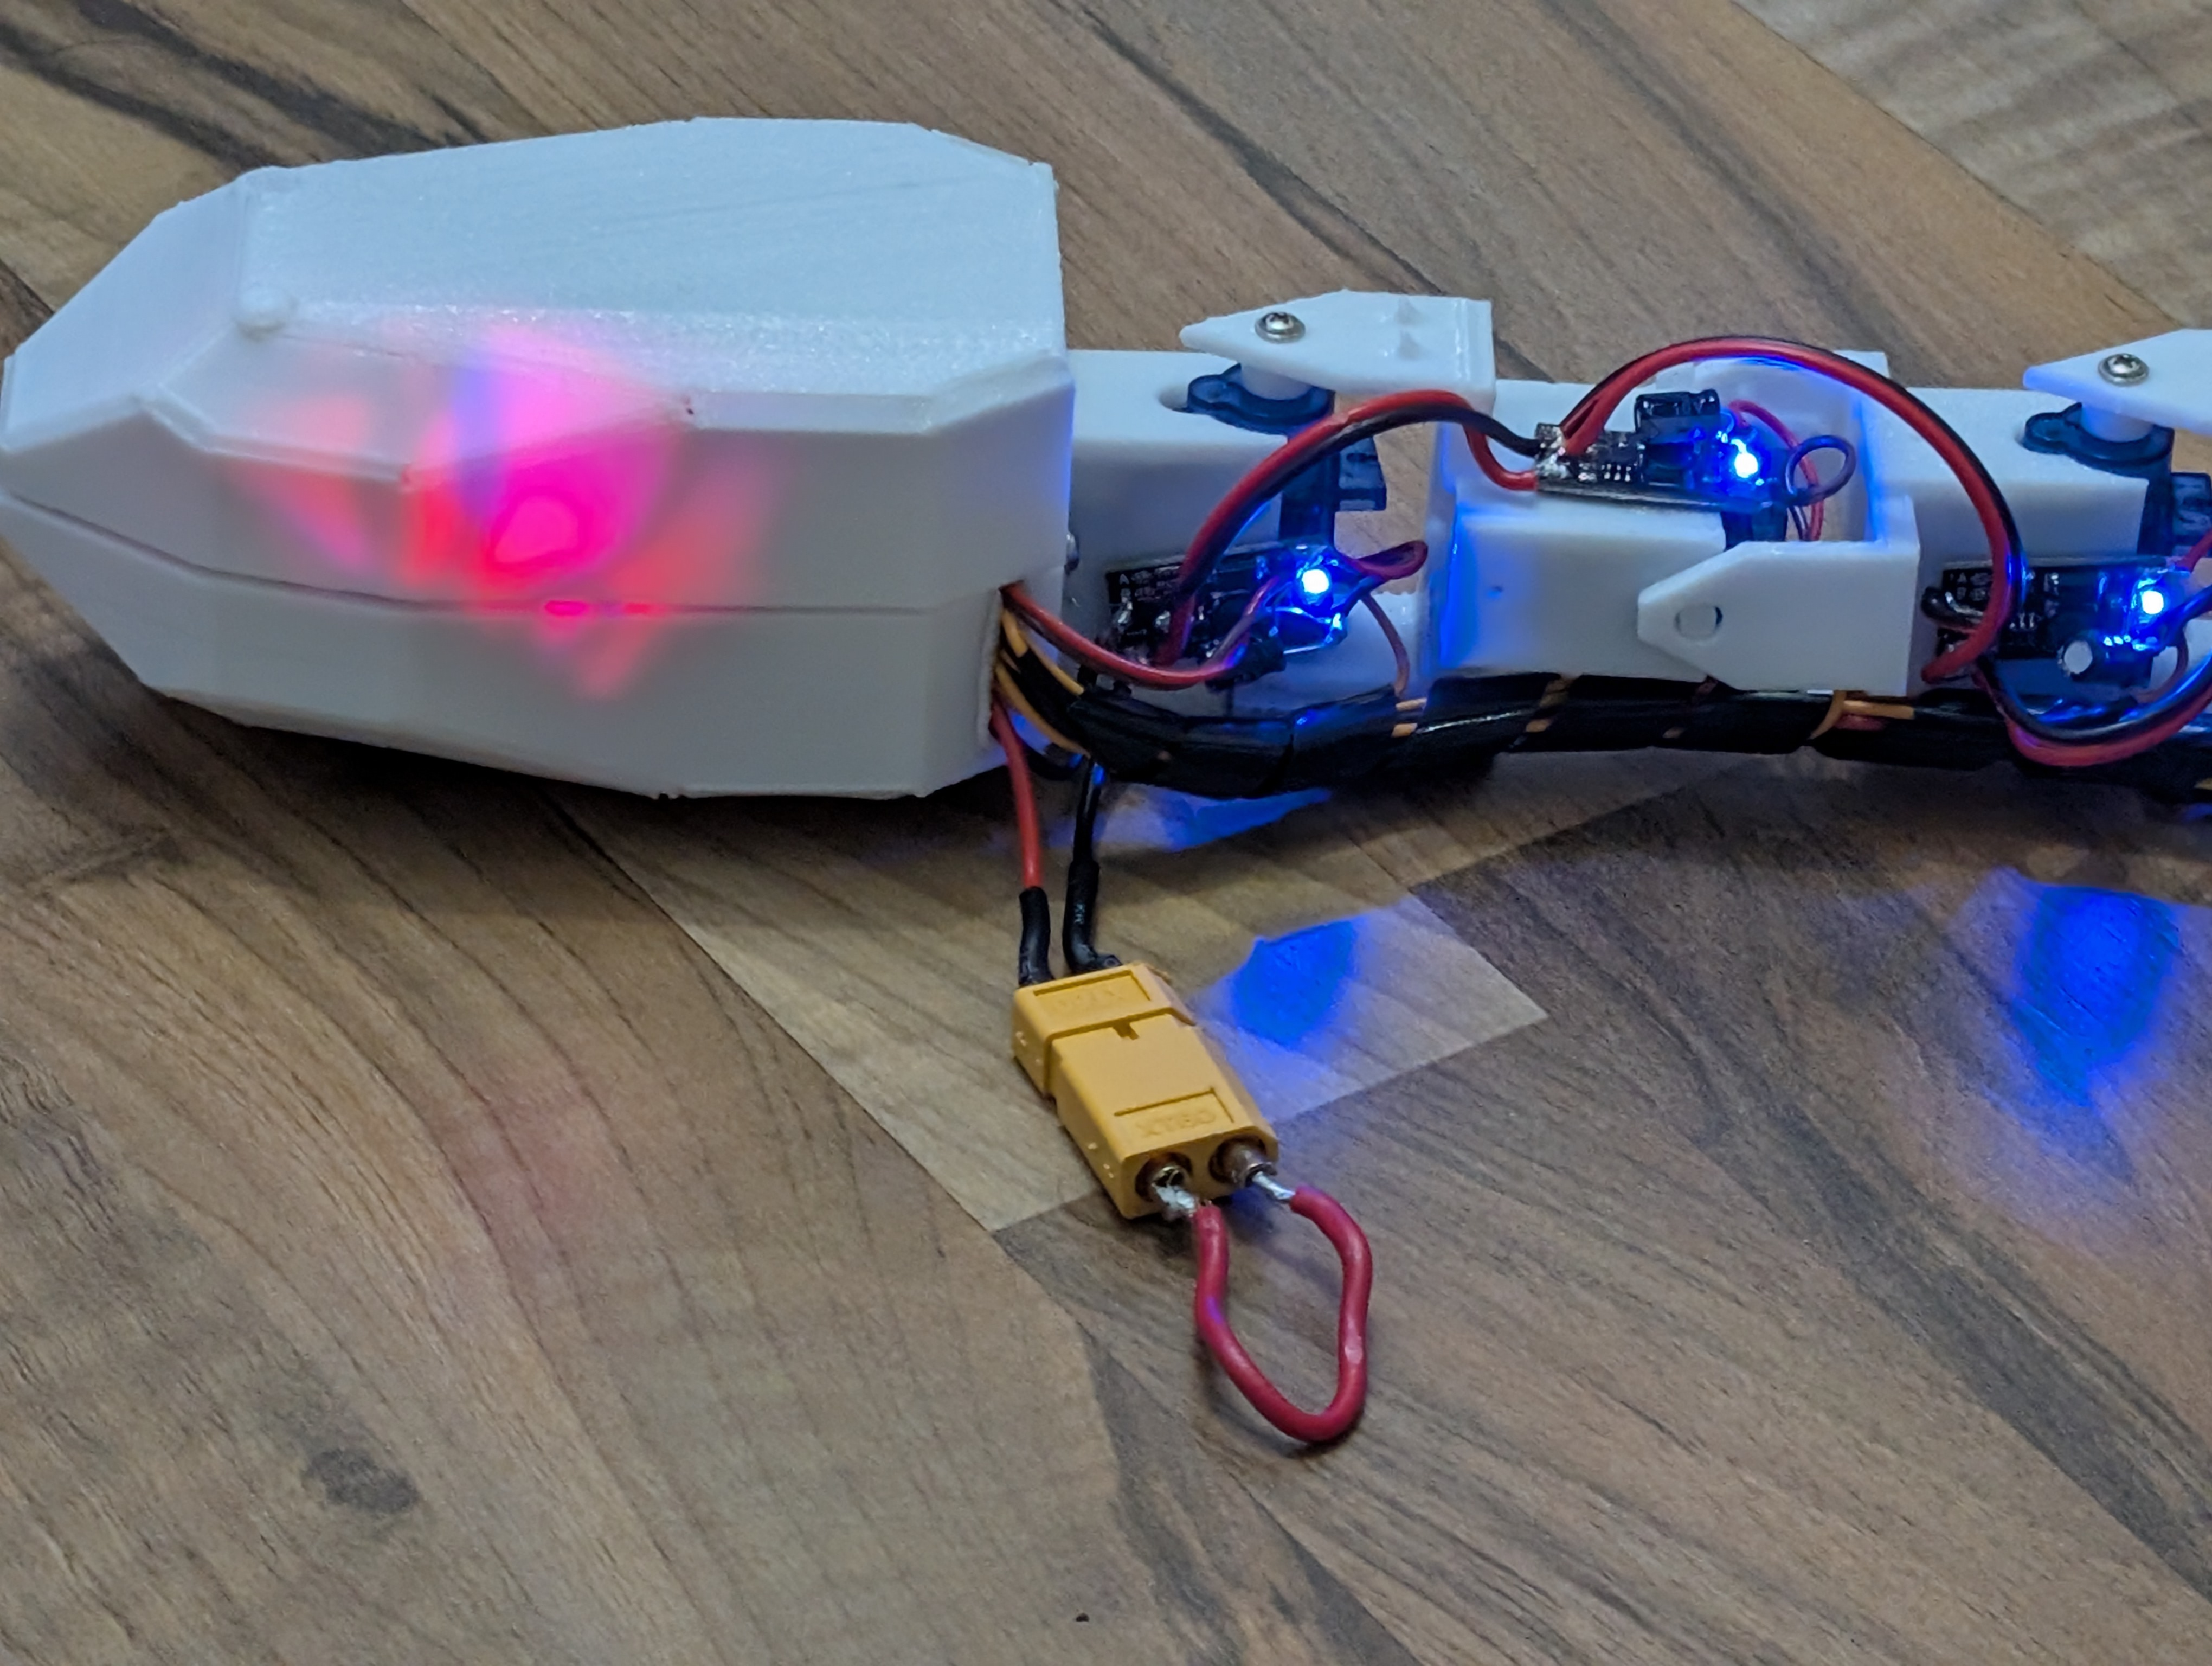
\includegraphics[width=0.3\textwidth]{media/snake_robot.jpg}
\end{titlepage}



\begin{abstract}
This thesis presents the design, implementation, and experimental evaluation of a neurobiologically inspired snake-like robot. Drawing from the locomotion mechanisms observed in biological snakes, the research develops a modular robotic system capable of executing multiple biologically authentic movement patterns. The work focuses on implementing Central Pattern Generator (CPG) inspired control algorithms to generate coordinated undulatory movements across the robot's segmented body. A 10-servo design with alternating horizontal and vertical actuation planes enables both lateral undulation and sidewinding locomotion patterns. The system utilizes an ESP32 microcontroller with WiFi connectivity to provide real-time control and parameter adjustment through a web-based interface. Three distinct robot configurations (baseline, with TPU-printed scales, and with PLA+ printed wheels) are experimentally evaluated to determine their effects on locomotion performance and energy consumption. Motion tracking analysis reveals differences in movement patterns between configurations, with wheels providing the most uniform progression during lateral undulation. Energy consumption measurements demonstrate that sidewinding requires more power than lateral undulation, and friction elements increase power requirements as well. The findings highlight the complex interplay between mechanical configuration, control parameters, and environmental interactions in biomimetic locomotion. This research contributes to the field of bioinspired robotics by providing insight into the design principles and control strategies for effective snake-like locomotion, with potential applications in search and rescue, pipeline inspection, and educational contexts.
\end{abstract}

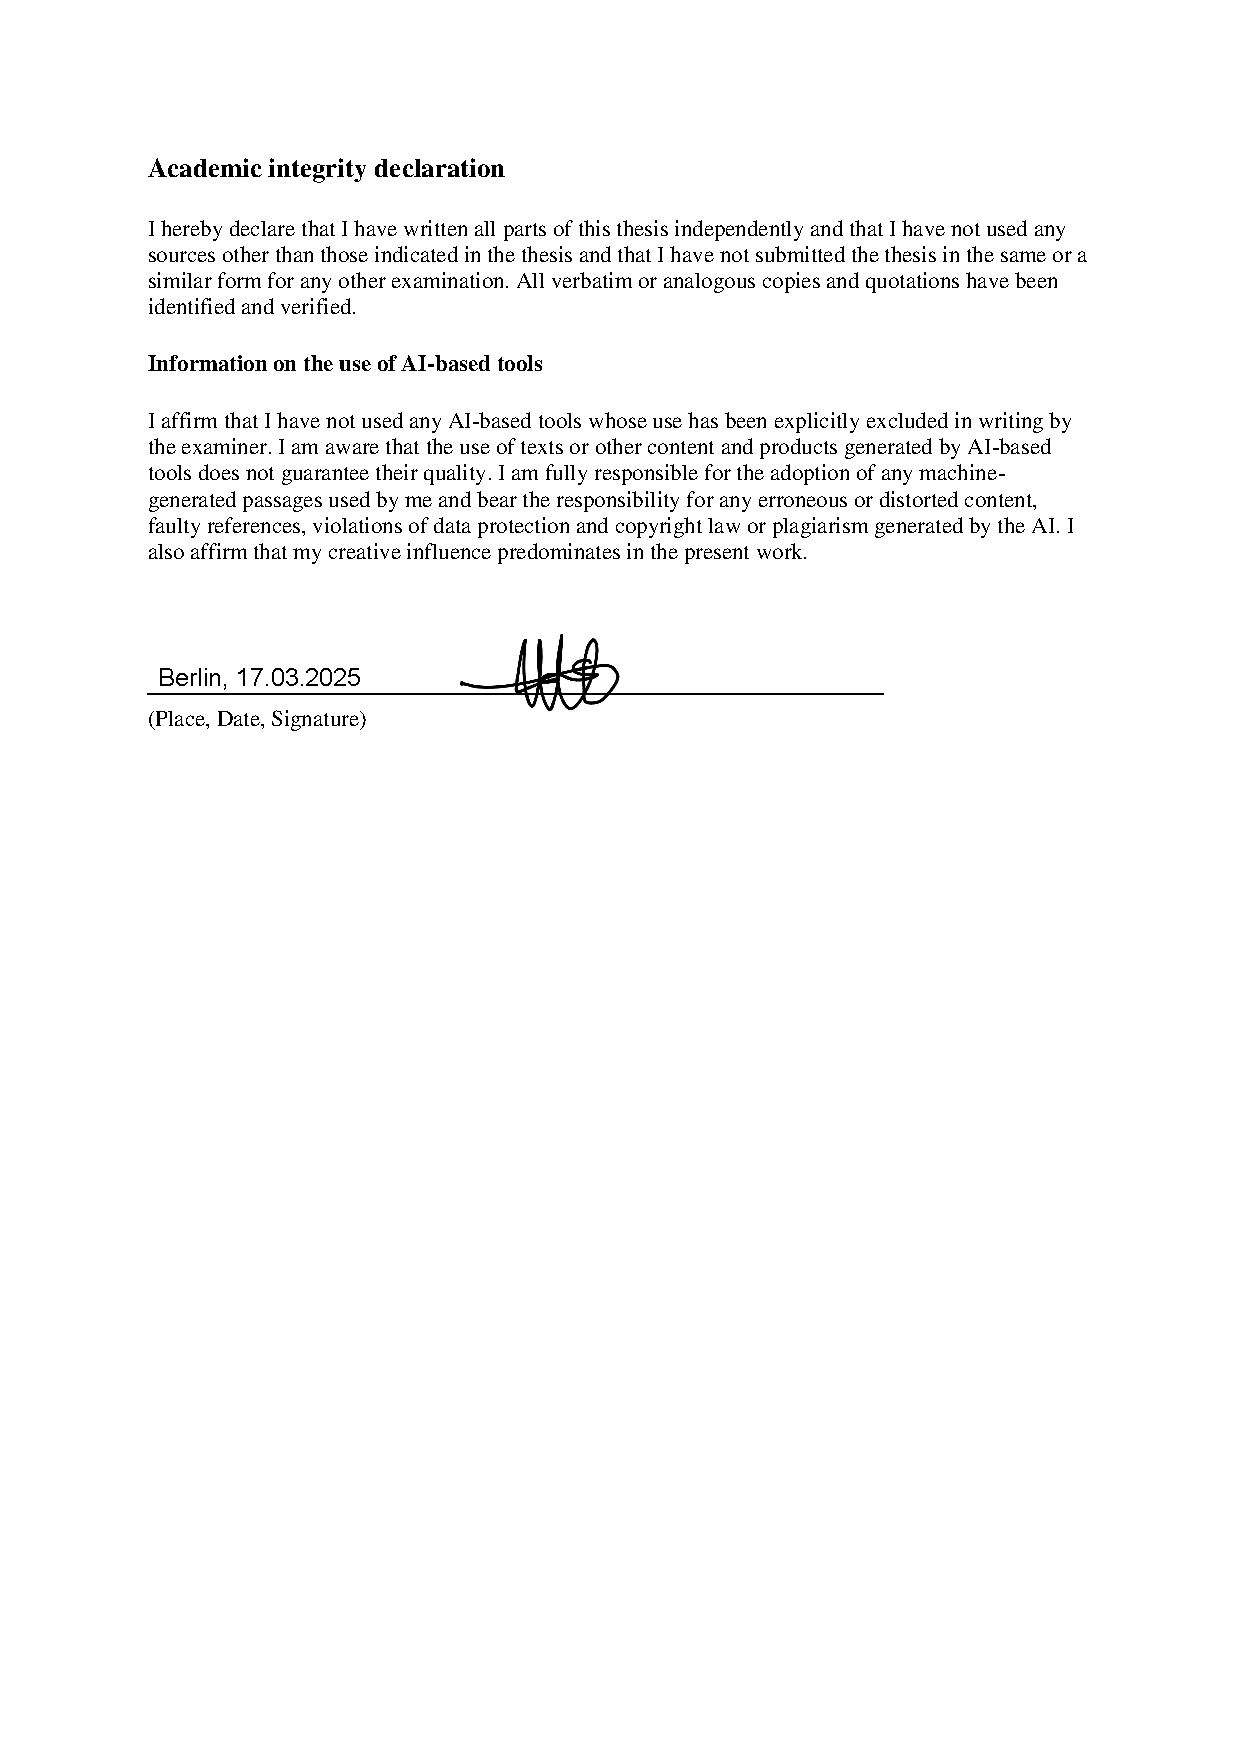
\includepdf[pages=-]{Eigenstaendigkeitserklaerung.pdf}
% Start Roman numeral page numbering
\pagenumbering{Roman}
% Table of Contents
\tableofcontents
\listoffigures
\newpage
\listoftables
\newpage
% Start Arabic numeral page numbering with Introduction
\cleardoublepage
\pagenumbering{arabic}
%//////////////////
%//////////////////
%chapter 1
%//////////////////
%//////////////////
\chapter{ Introduction}
Snake-like robots represent a fascinating intersection of biological inspiration and robotic engineering, offering unique mobility solutions for complex environments. This chapter establishes the foundation for understanding bio-inspired snake robotics, examining the research context, motivations, and key objectives that drive this field forward. 

\section{Background and Motivation}
Snake robots have emerged as a promising technological innovation inspired by the locomotion mechanisms observed in biological snakes. These robots exhibit exceptional adaptability in navigating confined spaces and overcoming challenging terrains where conventional wheeled or legged robots struggle. Their unique ability to generate smooth and continuous movements makes them particularly suitable for applications such as search-and-rescue missions, pipeline inspection, and medical procedures requiring minimally invasive interventions \cite{transeth-2009, Hirose2004}.

The fundamental advantage of snake-like robots lies in their ability to replicate the efficient and versatile locomotion strategies of real snakes. By leveraging undulatory movements, these robots can traverse irregular surfaces, maneuver through narrow gaps, and maintain stability on diverse terrain \textcite{Seeja2022}. The inspiration from biological systems, coupled with advances in robotic control, has led to significant progress in the field, paving the way for innovative robotic applications.

\section{Research Objectives}
This research aims to contribute to the development of bio-inspired snake robots by focusing on the following key objectives:

\begin{itemize}
    \item Design and construct a modular snake robot with multiple degrees of freedom to enable flexible and adaptive movement.
    \item Develop and optimize biologically inspired control algorithms to achieve efficient and stable locomotion.
    \item Implement and evaluate different motion patterns, including lateral undulation and serpentine locomotion, to enhance adaptability across various environments.
    \item Analyze the robot's performance metrics across different terrain types to assess its effectiveness and versatility.
    \item Integrate a robust hardware and software control system to ensure reliable operation and real-time adaptability in dynamic conditions.
\end{itemize}

\section{Paper Structure}
Following the introduction, this thesis proceeds with a chapter on the state of the art, covering biological principles of snake locomotion as well as the historical development and current research status on snake robots and CPG networks. The third chapter presents the system design and implementation of the snake robot, including mechanical construction using Onshape, 3D printing, and integration of the ESP32 microcontroller with ten servo motors. The fourth chapter details the experimental results, analyzing movement patterns and power consumption. Finally, the thesis concludes with a summary of research findings, limitations of the current implementation, and suggestions for future improvements. Supplementary technical documentation regarding hardware and software is provided in the appendix.

%//////////////////
%//////////////////
%chapter 2
%//////////////////
%//////////////////
\chapter{State of the Art}

This chapter reviews the biological principles of snake locomotion, including natural movement patterns and biomechanics. It also explores the historical development and current state of snake robot research, covering simulation and modeling approaches, biologically inspired robotic designs, and neurological models for locomotion control.

\section{Biological Snake Locomotion}
Snake locomotion has been extensively studied as a foundation for bio-inspired robotics. According to \textcite{liljeback-2013}, snake motion can be characterized by several distinct patterns, each optimized for different environmental conditions and objectives. These patterns have been widely implemented in robotic systems to improve their adaptability and efficiency in traversing complex environments.
Further investigations have examined the biomechanical principles underlying these motion patterns, contributing to the development of advanced control strategies \cite{lamping-2022}.

\subsection{Natural Snake Movement Patterns}
The primary motion patterns observed in biological snakes include:

\subsubsection{Lateral Undulation}
Lateral undulation, also known as serpentine motion, is the most common form of snake locomotion \textcite{liljeback-2013}. In this pattern, the snake creates a series of smooth curves that propagate from head to tail, generating forward thrust through the interaction with ground irregularities. \textcite{liljeback-2013} describe this as a wave-like motion where the snake's body follows the path traced by its head, with each segment of the body following the same spatial curve but with a time delay. 

\subsubsection{Rectilinear Motion}
According to \textcite{Zhenli2006} rectilinear locomotion occurs when "the skin of the ventral surface is moved forward and backward by strong muscles and the broad belly scales grip the ground, moving the snake forward in a straight line." The authors note that this form of locomotion "is used only by the heavier-bodied snakes."

\subsubsection{Concertina Locomotion} Concertina locomotion is named after a small accordion instrument, illustrating how the snake periodically folds and stretches its body to move forward. In this gait, the snake will anchor part of its body against the ground (or against a tunnel wall, tree branch, etc.), while other sections extend forward, after which the newly extended portion forms a new anchor and pulls the rest of the body along \cite{Zhenli2006}. note that this pattern is especially prevalent in constrained or narrow spaces, and it is often used for crossing smooth surfaces or climbing where other gaits may prove less effective.

\subsubsection{Sidewinding}
Sidewinding is "probably the most astonishing gait to observe and is mostly used by snakes in the desert" \cite{transeth-2009}. During this locomotion, "the snake lifts and curves its body leaving short, parallel marks on the ground while moving at an inclined angle" \cite{transeth-2009}. Unlike other gaits like lateral undulation, sidewinding involves "brief static contact between the body of the snake and the ground" \cite{transeth-2009}. This movement pattern is particularly useful "on surfaces with low shear such as sand" where snakes can achieve velocities up to 3 km/h \cite{transeth-2009}.

\subsection{Biomechanical Principles}
The effectiveness of snake locomotion relies on several key physical principles:

\subsubsection{Friction Models}
  As \textcite{lamping-2022} thoroughly analyze, anisotropic friction is crucial for effective snake movement. The contrast in forward versus reverse friction coefficients drives directional locomotion. This principle is significant for designing snake robots, which often require artificial scales or surface modifications to mimic this property. These mechanisms that enhance friction in snake-like robots are vital to improving their ability to adapt to a wide range of surfaces.
 
\subsubsection{Propulsion Mechanics}
The generation of propulsive forces in snake locomotion is achieved through strategic interactions with environmental push-points, where reaction forces contribute to forward movement. \textcite{Bayraktaroglu2006} describe how a snake-like robot mimics natural lateral undulation by utilizing push-points in the environment. Each module follows its predecessor, ensuring coordinated motion, while the orientation of reaction forces determines the overall direction of movement. The applied motor control inputs facilitate continuous progression similar to biological snakes.
Additionally, rhythmic motion patterns are regulated by neuronal circuits known as Central Pattern Generators (CPGs), described further in Section \ref{sec:neurological_models}.

\section{Snake Robots: State of the Art}

This section examines the evolution of snake robotics from its inception to current state-of-the-art implementations, highlighting key developments in mechanical design, control strategies, and application domains.

\subsection{Historical Development}
The historical evolution of snake robotics commenced with Hirose's pioneering work in 1972, developing the Active Cord Mechanism (ACM III), which became the foundational design for snake robots. Hirose introduced the concept of modularity and redundancy, emphasizing adaptability to challenging terrains through serpentine motion patterns \cite{transeth-2009}. His initial robot designs featured serially connected joints capable of undulatory locomotion, thus setting a standard for robust, modular robotic systems \cite{Hirose2004}.

Building upon Hirose's foundational contributions, research diversified into wheeled and wheel-less robotic designs. Initially, passive wheels were utilized to facilitate smooth movements on structured surfaces; however, these were limited to artificially prepared environments \cite{Bayraktaroglu2006}. Subsequently, a shift toward wheel-less snake robots was driven by a desire to replicate natural snake locomotion more accurately, leading to advancements in mechanical and control innovations \cite{transeth-2009}.

\subsection{Current Research Directions}
Contemporary research in snake robotics is focused on enhancing locomotion efficiency, adaptability, and control mechanisms. Several key areas of investigation include:

\subsubsection{Control Systems}

Central Pattern Generators (CPGs) have been increasingly applied to snake-like robots for generating rhythmic movements. \textcite{Seeja2022} discuss CPG-based algorithms enabling robots to dynamically adjust trajectories, facilitating obstacle avoidance and smooth turning motions. Sensory feedback integration further improves collision detection and adaptive movement capabilities.

\subsubsection{Alternative Locomotion Strategies}
\textcite{yamano-2023} propose a rolling motion strategy for snake-like robots that enhances efficiency by utilizing a shift in the center of gravity (COG). Their approach divides the rolling motion into four distinct phases: (1) the kick stage, where the robot’s head or tail moves to initiate ground contact and generate rolling motion; (2) COG shift stage I, in which a heavier link at the head or tail moves forward to reposition the COG; (3) COG shift stage II, where the same link is raised to further adjust the COG; and (4) the rolling stage, where gravity facilitates continuous rolling motion.

\subsubsection{Mechanical Design and Adaptability}
The impact of mechanical parameters, particularly scale angles and friction coefficients, on the locomotion of snake robots has been extensively studied. Research by \textcite{shen-2021} demonstrated that the angle of the robot’s scales can be dynamically adjusted using air pressure, directly influencing its movement efficiency. Their experiments revealed that an optimal anchoring coefficient is achieved when the scale angle is around 26.7° at a pressure of 12 kPa, significantly improving forward propulsion. Conversely, when the pressure exceeds 22 kPa, the scales flip direction, enabling backward locomotion. This adaptive approach mimics biological snake adaptations by altering surface friction to enhance traction and maneuverability.

\subsection{Simulation and Modeling}
Accurate modeling is essential for designing and optimizing snake robot locomotion. \textcite{liljeback-2013} provide a foundational analysis of lateral undulation, introducing a simplified dynamic model for control design and stability analysis. Their study highlights that effective locomotion control must incorporate time-varying strategies, as static control laws fail to stabilize the system due to its inherent dynamics. Using averaging theory, they derived fundamental relationships between gait parameters and forward velocity, showing that the robot’s motion can be analytically predicted and optimized based on these parameters. This work has been instrumental in developing physics-based simulations that enable rapid prototyping and validation of locomotion strategies.

An additional contribution to simulation methodologies comes from \textcite{yogesh2023snake}, who provides open-source simulation tools for snake robot modeling. These practical implementations facilitate experimentation with different control strategies and locomotion patterns, supporting researchers in optimizing robot performance before physical deployment.

\subsection{Biologically Inspired Snake-like Robots}
Bio-inspired design principles continue to drive innovations in snake robotics. \textcite{Mohammed2016} developed a 3D printed modular snake robot that integrates flexible joint structures, enhancing both maneuverability and robustness. Their research highlights the benefits of modularity, where each module functions as a single rotational joint with one degree of freedom (DOF). The robot's structure allows for movement across multiple axes, enabling adaptability in various applications, such as search-and-rescue and medical robotics.

Building on this, \textcite{Arachchige2021} explored the potential of soft robotic snakes (SRS) by incorporating spatial bending capabilities to extend locomotion beyond conventional planar gaits. Their study demonstrates how continuous and smooth bending enables snake robots to better replicate biological movement, allowing for improved adaptability in climbing, swimming, and traversing complex terrains. These advancements highlight how soft robotics principles enhance maneuverability while maintaining structural integrity and operational efficiency.

\section{Neurological Models of Snake Locomotion}
\label{sec:neurological_models}
The locomotion of snakes has been extensively studied, revealing that their movement is governed by neural circuits that enables adaptive and rhythmic motion. This capability is controlled by Central Pattern Generators (CPGs), which are neural circuits responsible for generating rhythmic outputs without requiring continuous sensory feedback. These circuits, located within the spinal cord, play a fundamental role in orchestrating rhythmic behaviors such as walking, swimming, and crawling in both vertebrates and invertebrates \cite{MARDER2001R986}

\subsection{Central Pattern Generator (CPG) Model}

CPGs, fundamental to locomotion control, are extensively modeled to replicate the rhythmic patterns of snake locomotion. They typically comprise coupled neural oscillators that produce rhythmic signals with stable oscillations and phase-shifted outputs for coordinated joint movements \cite{wang2020cpg}. Various approaches to CPG modeling have been proposed:

\FloatBarrier
\subsubsection{Mutual Inhibitory CPGs}

One of the fundamental architectures for generating rhythmic motion is the mutual inhibitory CPG model shown in Figure~\ref{fig:mutual_inhibitory_cpg}, which consists of neuron pairs that reciprocally inhibit each other, leading to stable oscillations. This architecture ensures continuous rhythmic movement. However, it lacks adaptability to environmental variations because it does not inherently produce sustained oscillations without additional adaptation mechanisms \cite{Lu2006}.

\begin{figure}[H]
\centering
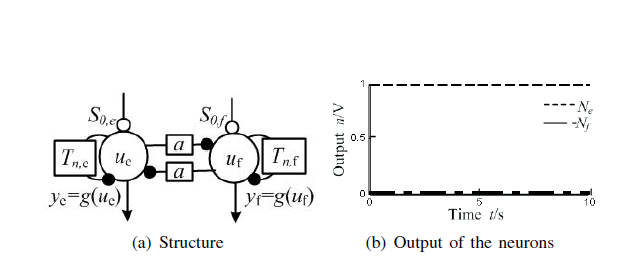
\includegraphics[width=0.5\textwidth]{media/MI_CPG.png}
\caption{Mutual inhibitory CPG model \cite{Lu2006}. This model illustrates pairs of neurons reciprocally inhibiting each other, creating stable rhythmic oscillations.}
\label{fig:mutual_inhibitory_cpg}
\end{figure}

\subsubsection{Cyclic Inhibitory CPGs}

Cyclic inhibitory CPG models address the limitations of mutual inhibitory architectures by incorporating feedback loops that enable the system to maintain oscillatory activity over time. These models involve interconnected neurons in a cyclic inhibitory structure (see Figure \ref{fig:cyclic_inhibitory_cpg}), allowing for sustained and coordinated oscillations. This design proves particularly effective in generating stable 3D locomotion, as it enhances phase synchronization across multiple joints. Studies have demonstrated the effectiveness of this model in achieving robust serpentine motion, making it a preferable choice for controlling the locomotion of snake-like robots \cite{Lu2006}.

\begin{figure}[H]
\centering
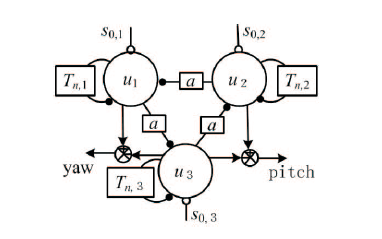
\includegraphics[width=0.5\textwidth]{media/CI_CPG.png}
\caption{Cyclic inhibitory CPG model \cite{Lu2006}}
\label{fig:cyclic_inhibitory_cpg}
\end{figure}

\subsubsection{Sensory Feedback-Integrated CPGs}
Recent advancements in CPG modeling incorporate sensory feedback mechanisms, allowing adaptive locomotion. These models integrate sensory information through sensory interneurons (SIN), which relay environmental data back to the CPG, enabling real-time adjustments to oscillatory parameters \cite{Inoue2007}. For instance, \textcite{Inoue2007} implemented a CPG-based control system where sensory input was processed by SIN and fed back into the CPG, enhancing the robot's ability to adapt to variations in ground friction.

\subsubsection{Evolutionary and Learning-Based CPGs}
Machine learning and evolutionary algorithms have been applied to optimize CPG parameters for snake locomotion. By employing genetic algorithms (GA), researchers have enabled robots to autonomously refine their locomotion patterns in response to different terrains and obstacles \cite{Inoue2007}. Specifically, \textcite{Inoue2007} used GA to evolve CPG parameters that maximize adaptability across varying friction conditions, demonstrating that multi-environment performance-based evaluation functions enhance adaptive locomotion.

\subsection{Implementation Considerations}
When implementing CPG-based control, several key factors must be considered:
\begin{itemize}
    \item Phase Relationships Between Segments: To achieve effective serpentine locomotion, it is essential to maintain a consistent phase difference between joint oscillations. This phase control ensures synchronized movement, allowing the robot to generate propulsion force through interactions with the ground \cite{Norzalilah2014}.
    \item Coupling Strengths Between Oscillators: The coordination between different segments of a CPG network is influenced by the strength of the connections between oscillators. Proper tuning of descending and ascending coupling pathways is necessary to ensure segmental synchronization, which requires detailed anatomical and electrophysiological studies \cite{MARDER2001R986}.
    \item Adaptation Mechanisms for Environmental Feedback: A robust CPG-based system must integrate sensory feedback to adapt to environmental variations. Sensory inputs, such as ground reaction forces or muscle length changes, can be fed back into the CPG network to enhance stability and improve locomotion resilience against disturbances \cite{Inoue2007}.
    \item Stability of Rhythm Generation: The stability of rhythmic motion depends on ensuring bounded and well-defined oscillatory behavior. Mathematical conditions such as Lipschitz continuity help establish the existence and uniqueness of stable rhythmic solutions in CPG models, preventing disruptions in locomotion patterns \cite{Zhenli2006}.
\end{itemize}

These models provide a foundation for developing bio-inspired control systems that can generate smooth, coordinated motion patterns while maintaining adaptability to environmental changes.

\subsection{Mathematical Representation of CPG Networks}

The neural control system of a snake-like robot can be mathematically modeled as a network of coupled oscillators. As described by \textcite{wang2020cpg}. each oscillator in the network represents a segmental neural circuit. The system is structured as a single-chain bidirectional coupling network, where each connection between oscillators is defined by a phase lag parameter. The network's dynamics are governed by the following set of differential equations:

\begin{equation}
    \dot{\theta}_k =
    \begin{cases} 
        2\pi v + w \sin(\theta_2 - \theta_1 + \phi), & k = 1 \\
        2\pi v + w \left[\sin(\theta_{k-1} - \theta_k - \phi) + \sin(\theta_{k+1} - \theta_k + \phi)\right], & 2 \leq k \leq N-1 \\
        2\pi v + w \sin(\theta_{N-1} - \theta_N - \phi), & k = N
    \end{cases}
\end{equation}

where \( \theta_k \) represents the phase of the \( k \)-th oscillator, \( v \) denotes the intrinsic oscillation frequency, and \( w \) is the coupling strength between oscillators. The output of each oscillator, corresponding to the joint angle in a snake-like robot, is given by:

\begin{equation}
    \phi_k = A \cos(\theta_k), \quad 1 \leq k \leq N
\end{equation}

where \( A \) represents the oscillation amplitude. This mathematical formulation provides a precise method for generating rhythmic movement, crucial for implementing bio-inspired locomotion strategies in snake-like robots \cite{wang2020cpg}.

%//////////////////
%//////////////////
%chapter 3
%//////////////////
%//////////////////

\chapter{System Design, Implementation, and Details}

This chapter presents the complete design and implementation of the bio-inspired snake robot, focusing on its hardware architecture, control system, and motion generation. Inspired by biological snake locomotion patterns, the system employs Central Pattern Generator (CPG)-based control strategies.


\section{Evolution of System Design}
The snake robot underwent several iterations, each driven by practical testing and the desire to overcome early design limitations. The first prototype was built around an STM32-L432KC microcontroller with only preprogrammed parameters, offering no interface to start, stop, or adjust the locomotion algorithm in real time. All circuitry, including the buck converters, was centralized in the head module, making it disproportionately large and heavy compared to the rest of the body. This imbalance placed excessive strain on the front servo motor, reducing maneuverability and overall efficiency.

Motivated by these limitations, a new approach centered on the ESP32 microcontroller was adopted. The ESP32 not only offers more capable processing but also provides built-in wireless connectivity, allowing for a WiFi-based interface to control motion parameters remotely. Beyond WiFi, the ESP32 facilitates future expansion via ESP-NOW for direct controller-to-controller links, making it possible to develop a dedicated handheld remote or integrate additional sensing modules without physical wiring. Familiarity with the ESP32 development environment and libraries further justified its selection over the STM32 platform.

In parallel with changing the microcontroller, the mechanical design was refined to address structural weaknesses. Rather than relying on a single contact point in each joint, two robust contact points were introduced, significantly improving stability and mitigating stresses that lead to early mechanical failures. A vertical joint was also added to enable out-of-plane motion, expanding the robot’s maneuverability beyond simple horizontal undulations and paving the way for more complex locomotion strategies.

\subsection{Distributed Power and Noise Mitigation}
Shifting the power architecture to a distributed design represented another key enhancement. Instead of locating all buck converters in the head, individual converters were placed near each servo motor. This arrangement reduced the length and complexity of wiring, requiring only a single power line routed from the battery to each converter. Although this layout made the design cleaner and lighter, it also introduced an issue with signal noise: the servos occasionally moved erratically or exhibited jitter.

A detailed investigation revealed that the combination of servo control signals and distributed power lines led to unwanted interference. To counteract this noise, a 16\,V/100\,$\mu$F capacitor was placed on each buck converter output, acting as a local power reservoir. Additionally, each servo signal line was equipped with a 10\,k$\Omega$ pull-down resistor, which helped stabilize the control signals. These hardware modifications effectively eliminated the jitter and restored precise servo actuation.

\subsection{Battery Selection and Current Sensing}
After refining the cabling and completing initial motion tests, it became evident that the chosen battery’s built-in current-limiting protection would occasionally trigger and power down the system. During peak load conditions, especially when multiple servos actuated simultaneously, the protection circuit perceived an overcurrent event and disconnected the output. 

To address this, a standard 18650 Li-ion cell without built-in current-limiting circuitry was chosen as the primary power source. Realizing that accurate power monitoring would be critical, an ACS712-based current sensor was integrated into the design. By measuring the instantaneous current draw, the control software can monitor power consumption in real time, log average and peak current usage, and provide valuable diagnostics to the user. 

\section{Hardware Implementation}
Following the above design decisions, the mechanical and electronic structures were consolidated into a modular system. The head module now houses the ESP32, the main battery, the current sensor, and the primary wiring harnesses routed through a dedicated cable management channel. Buck converters are distributed such that each servo has a nearby power regulator, ensuring stable voltage supply and reducing the chance of voltage drops or noise accumulation.

Mechanically, each segment features two robust hinge contact points to support lateral and vertical movements. A vertical joint segment is inserted at intervals to allow out-of-plane motion, enhancing maneuverability beyond simple sinusoidal undulation. The tail segment carries no electronics and adds more of a Visual effect than a practical one.

\section{Control System Architecture}
Leveraging the ESP32’s computing and connectivity, the control system adopts a bio-inspired Central Pattern Generator (CPG) approach to coordinate the robot’s undulations. The CPG model allows for parameterized control over amplitude, phase offset, and frequency, all of which can be modified in real time via a web-based interface hosted directly on the ESP32.

During operation, the ESP32 creates an access point through which a user can connect via a standard web browser. Motion parameters, start/stop commands, and other real-time adjustments are transmitted via HTTP POST requests, immediately influencing the CPG outputs and servo drive signals. This wireless interface greatly simplifies experimentation with different locomotion patterns, as it eliminates the need for physical programming cables and manual adjustments.

Future expansions include employing ESP-NOW to link the snake robot’s ESP32 with a remote-control unit, also based on an ESP32, enabling direct, low-latency communication. This setup could further extend to multiple sensory modules or even swarm collaboration between multiple robots. In summary, the move to an ESP32 platform, combined with distributed power regulation, vertical joint integration, and robust noise suppression, has significantly enhanced both the mechanical and electronic performance of the snake robot while laying a flexible foundation for continued innovation.

\begin{figure}[h]
\centering
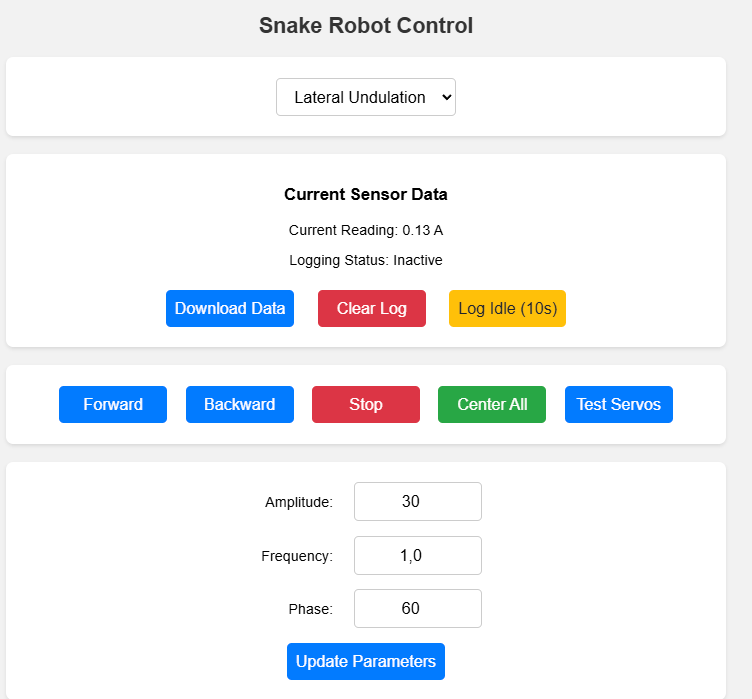
\includegraphics[width=0.5\textwidth]{media/WebUi.png}
\caption{Web Ui to control the snake's behavier}
\end{figure}

\section{Motion Pattern Generation}
Locomotion is generated using biologically inspired Central Pattern Generator (CPG) algorithms, primarily implementing lateral undulation and sidewinding patterns. The control system is designed to mimic the neurobiological motion generation found in biological snakes, where rhythmic patterns emerge from neural networks without requiring continuous sensory feedback \parencite{MARDER2001R986}. 

\subsection{Lateral Undulation}
Lateral undulation is the most common locomotion pattern observed in biological snakes and is particularly effective on flat surfaces with friction \parencite{transeth-2009}. In our implementation, this pattern follows a traveling wave function, where each servo's angular displacement is determined by a sinusoidal function:

\begin{equation}
\theta_i(t) = A \sin(\omega t + \phi_i) + \theta_{\text{offset}}
\end{equation}

Where:
\begin{itemize}
    \item $\theta_i(t)$ is the angle of the $i$-th servo at time $t$,
    \item $A$ is the amplitude of the wave (controlled via the interface as \texttt{amplitude}),
    \item $\omega = 2\pi f$ is the angular frequency based on frequency $f$ (controlled as \texttt{frequency}),
    \item $\phi_i$ is the phase offset for the $i$-th segment, calculated as $i \cdot \text{phaseOffset}$,
    \item $\theta_{\text{offset}}$ is the center position (set to 90° in our implementation).
\end{itemize}

Looking at the implementation, the lateral undulation is generated in the \break \texttt{updateServosLateralUndulation()} function. The time-dependent parameter is calculated as:

\begin{equation}
\text{timeScale} = t \cdot 0.001 \cdot f \cdot 2\pi
\end{equation}

Where $t$ is the system time in milliseconds from the \texttt{millis()} function, scaled to seconds with the 0.001 factor. This provides the temporal component of the wave.

For each horizontal servo in the array, a phase offset is applied depending on the segment's position and the desired direction of travel:

\begin{equation}
\text{segmentPhase} = 
\begin{cases}
(N_h - 1 - i) \cdot \phi & \text{for forward motion} \\
i \cdot \phi & \text{for backward motion}
\end{cases}
\end{equation}

Where $N_h$ is the number of horizontal servos (7 in our implementation), $i$ is the index of the horizontal servo, and $\phi$ is the phase offset in radians. The inversion of phase progression for different directions creates a traveling wave that moves either anteriorly or posteriorly along the robot's body, similar to how biological snakes propagate waves from head to tail during forward motion \parencite{liljeback-2013}.

The final angular position of each servo is calculated as:

\begin{equation}
\theta_i = \theta_{\text{center}} + A \cdot \sin(\text{timeScale} + \text{segmentPhase})
\end{equation}

An important consideration in our implementation is that the phase relationship definition for forward and backward motion is carefully constructed to ensure the wave propagates in the correct direction. For forward motion, the wave must travel from the tail toward the head (posteroanterior propagation), creating a pushing force against the ground that propels the robot forward. Our implementation achieves this by inverting the phase index calculation for forward motion, ensuring the wave propagates in the correct biological direction.


\begin{figure}
  \centering
  \animategraphics[controls,width=0.8\textwidth]{12}{media/Lateral/ezgif-frame-}{1}{33}
  \caption{Lateral Undulation simulation showing the propagation of the sinusoidal wave through the robot's body. Note how the wave travels from tail to head during forward motion.}
  \label{fig:lateral-anim}
\end{figure}

\FloatBarrier
\subsection{Sidewinding}
Sidewinding is a more complex locomotion pattern used by snakes in low-friction environments such as sand or smooth surfaces \cite{transeth-2009}. It combines horizontal and vertical wave motions with a specific phase relationship between them to generate a lifting effect. This implementation follows concepts from studies like \textcite{yamano-2023} and is formulated as:

\begin{equation}
\theta_{i,h}(t) = A_h \sin(\omega t + \phi_{i,h}) + \theta_{\text{center}}
\end{equation}

\begin{equation}
\theta_{i,v}(t) = A_v \sin(\omega t + \phi_{i,v} + \Delta\phi) + \theta_{\text{center}}
\end{equation}

Where:
\begin{itemize}
    \item $\theta_{i,h}(t)$ represents the horizontal actuation of the $i$-th servo,
    \item $\theta_{i,v}(t)$ represents the vertical actuation,
    \item $A_h$ and $A_v$ are the respective amplitudes of horizontal and vertical motion (set as \texttt{amplitude} and \texttt{verticalAmplitude} in our implementation),
    \item $\phi_{i,h}$ and $\phi_{i,v}$ are the phase offsets for each segment,
    \item $\Delta\phi$ is the phase difference between horizontal and vertical waves (set to 90° in our implementation).
\end{itemize}

The implementation in \texttt{updateServosSidewinding()} handles both horizontal and vertical servos differently. For horizontal servos, the phase calculation considers the direction of travel:

\begin{equation}
\phi_{i,h} = 
\begin{cases}
(N_h - 1 - i) \cdot \phi & \text{for forward motion} \\
i \cdot \phi & \text{for backward motion}
\end{cases}
\end{equation}

For vertical servos, the phase relationship includes both the progressive phase based on segment position and the additional vertical phase offset:

\begin{equation}
\phi_{i,v} = 
\begin{cases}
(N_v - 1 - i) \cdot \phi + \phi_{\text{vertical}} & \text{for forward motion} \\
i \cdot \phi + \phi_{\text{vertical}} & \text{for backward motion}
\end{cases}
\end{equation}

Where $N_v$ is the number of vertical servos (3 in our robot), $i$ is the index of the vertical servo, $\phi$ is the phase offset, and $\phi_{\text{vertical}}$ is the additional phase offset between horizontal and vertical waves (set to 90° or $\pi/2$ radians).

This configuration creates a coordinated lifting and lateral movement that allows the robot to "sidestep" across surfaces. The vertical wave component causes segments to lift off the ground in sequence, while the horizontal component creates the necessary lateral displacement. The 90° phase difference between the horizontal and vertical waves is critical, as it ensures that maximum vertical displacement occurs at the appropriate point in the horizontal cycle \parencite{yamano-2023}.

Our specific implementation of the vertical servo control in sidewinding uses a more complex phase calculation that accounts not only for the segment position but also adjusts for the direction of travel. For forward motion, the phase progression is inverted similarly to the horizontal servos, but with an adjustment for the different number of vertical servos:

\begin{equation}
\phi_{i,v} = (N_t - N_h - 1 - i) \cdot \phi + \phi_{\text{vertical}}
\end{equation}

Where $N_t$ is the total number of servos (10) and $N_h$ is the number of horizontal servos (7). This ensures proper coordination between horizontal and vertical movements during direction changes.


\begin{figure}
  \centering
  \animategraphics[controls,width=0.8\textwidth]{12}{media/Side/ezgif-frame-}{1}{33}
  \caption{Sidewinding movement simulation showing the combined effect of horizontal and vertical wave propagation. Note the diagonal lifting pattern that creates the characteristic sidewinding motion.}
  \label{fig:side-anim}
\end{figure}

\subsection{Servo Layout and Configuration}
The physical arrangement of servos in our snake robot follows a specific pattern designed to support both locomotion modes effectively. The robot consists of 10 servo modules arranged in an alternating pattern of horizontal and vertical actuators:

\begin{equation}
\text{servoLayout} = [1, 0, 1, 1, 0, 1, 1, 0, 1, 1]
\end{equation}

Where 1 represents a horizontal servo (7 total) and 0 represents a vertical servo (3 total). This asymmetric distribution was chosen based on preliminary testing that showed better performance with more horizontal actuators, while still providing sufficient vertical control for effective sidewinding.

\begin{figure}
  \centering
  \includesvg[width=0.9\textwidth]{media/svg/Layout_Diagram.svg}
  \caption{Physical arrangement of servos in the snake robot showing the alternating pattern of horizontal (H) and vertical (V) actuators. The diagram illustrates how each servo's axis of rotation contributes to the overall motion pattern.}
  \label{fig:servo-layout}
\end{figure}

\subsection{Parameter Control and Adaptation}
The implementation allows for real-time adjustment of key locomotion parameters through the web interface:

\begin{itemize}
    \item \textbf{Amplitude}: Controls the maximum angular displacement of servos (10°-45°)
    \item \textbf{Frequency}: Determines the speed of wave propagation (0.1-2.0 Hz)
    \item \textbf{Phase Offset}: Sets the phase difference between adjacent segments (30°-90°)
\end{itemize}

These parameters can be adjusted to optimize the robot's movement across different surfaces and conditions. The interface constrains these values within practical ranges to ensure stable locomotion while preventing mechanical stress on the servos.

Our implementation uses the constrain() function to ensure parameters remain within safe operating ranges:

\begin{equation}
\text{amplitude} = \text{constrain}(\text{amplitude}, 10.0, 45.0)
\end{equation}

\begin{equation}
\text{frequency} = \text{constrain}(\text{frequency}, 0.1, 2.0)
\end{equation}

\begin{equation}
\text{phaseOffset} = \text{constrain}(\text{phaseOffset}, 30.0, 90.0)
\end{equation}

The effects of these parameters on locomotion performance are illustrated in Figure \ref{fig:param-effects}.

\subsection{Implementation of CPG Network}
While traditional CPG implementations often use coupled oscillator networks, 
% \parencite{wang2020cpg}
 our approach uses a simplified mathematical model that achieves equivalent functionality. The sinusoidal wave generation with appropriate phase relationships effectively simulates the output of a CPG network, where:

\begin{equation}
\text{CPG}_i(t) = \sin(\omega t + \phi_i)
\end{equation}

This approach is computationally efficient while still capturing the essential characteristics of biological CPGs. The phase relationships between segments create an interconnected system similar to the coupled oscillators in biological neural circuits.

The update frequency of the motion generation system is set to 50 Hz (with an interval of 20 ms), ensuring smooth motion while being well within the processing capabilities of the ESP32 microcontroller. This frequency is sufficient to maintain fluid, continuous movement patterns while allowing for other system operations such as handling web server requests and data logging.

\subsection{Direction Control}
The direction of travel is controlled by inverting the phase progression along the body. For forward motion, the phase offset increases from head to tail, while for backward motion, the phase progression is reversed. This mimics the biological control strategy in which the direction of wave propagation determines the direction of movement.

In the implementation, this is achieved through conditional logic in both locomotion functions that selects the appropriate phase calculation based on the \texttt{forwardDirection} boolean variable. This direction control is critical for both locomotion patterns, though the specific implementation differs slightly between lateral undulation and sidewinding to account for the different servo configurations and wave propagation patterns.

A key insight from our implementation is that a critical factor for effective direction control is ensuring the proper relationship between the direction of wave propagation and the desired movement direction. For lateral undulation, forward motion requires a posteroanterior wave (tail to head), while backward motion requires an anteroposterior wave (head to tail).
%//////////////////
%//////////////////
%chapter 4
%//////////////////
%//////////////////
\chapter{Experimental Results and Analysis}
This chapter presents the performance evaluation of the snake robot. It includes detailed analyses of the movement, and testing with different friction modules. Specific evaluations include motion pattern analysis and power consumption.

\section{Experimental Setup}
To evaluate the performance of the neurobiologically inspired snake robot, a series of experiments was conducted under controlled conditions. The primary objective was to assess the different locomotion patterns and analyze how various robot configurations influence movement capabilities.

\subsection{Testing Environment}
All experiments were conducted on laminate wood flooring, providing a low-friction, uniform surface for consistent testing conditions. For quantitative movement analysis, a testing area was created using:
\begin{itemize}
    \item A horizontal strip of cardboard extending 130 cm, marked with tape at 10 cm intervals
    \item A vertical strip of cardboard extending 70 cm, marked with tape at 10 cm intervals
\end{itemize}

This grid setup enabled precise tracking of the robot's two-dimensional movement path, providing reference points for subsequent video analysis. The grid layout is illustrated in Figure~\ref{fig:tracking_setup}.

\begin{figure}[H]
    \centering
    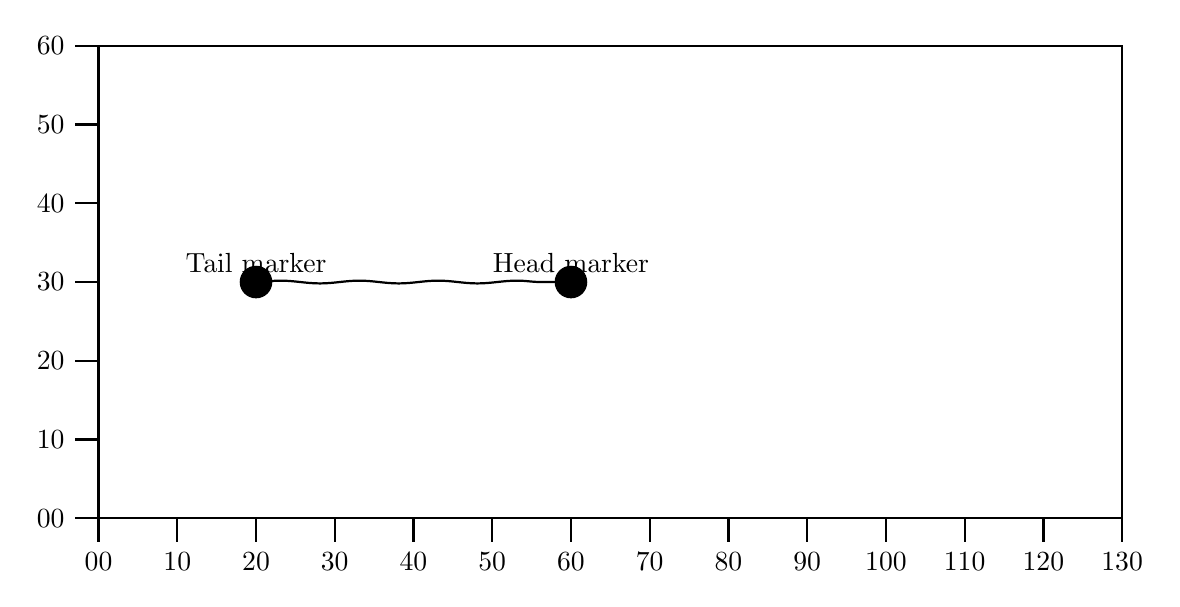
\begin{tikzpicture}
        % Draw the testing area
        \draw[thick] (0,0) rectangle (13,6);
        
        % Draw horizontal markers
        \foreach \x in {0,1,...,13}
            \draw[thick] (\x,0) -- (\x,-0.3) node[below] {\x0};
        
        % Draw vertical markers
        \foreach \y in {0,1,...,6}
            \draw[thick] (0,\y) -- (-0.3,\y) node[left] {\y0};
        
        % Draw snake robot schematically
        \draw[thick, snake=snake, segment amplitude=0.5, segment length=1cm] (2,3) -- (6,3);
        
        % Draw tracking markers
        \filldraw[black] (2,3) circle (0.2) node[above] {Tail marker};
        \filldraw[black] (6,3) circle (0.2) node[above] {Head marker};
    \end{tikzpicture}
    \caption{Experimental setup showing the testing area with measurement grid and tracking markers on the snake robot.}
    \label{fig:tracking_setup}
\end{figure}

\begin{figure}[h]
\centering
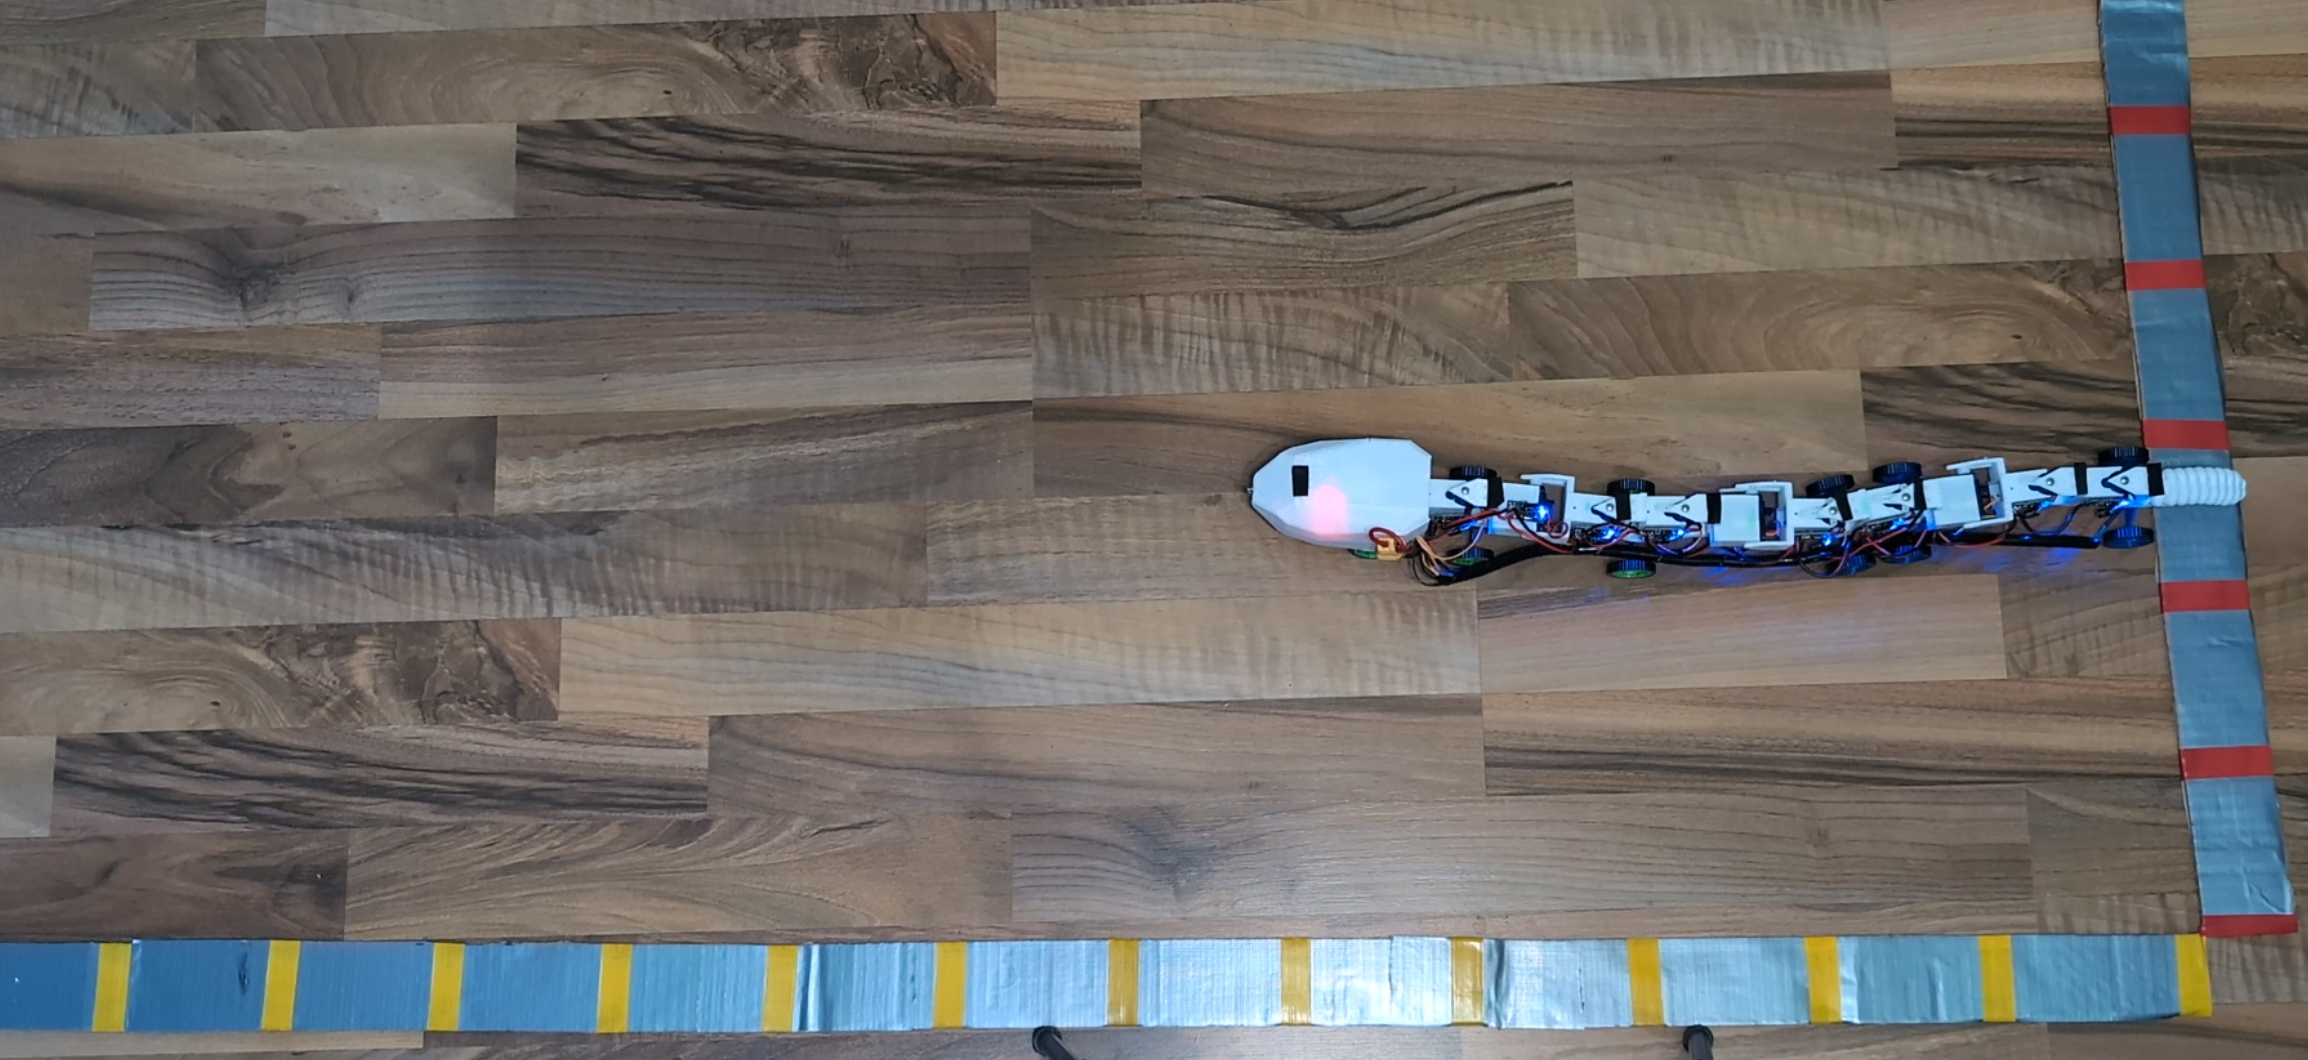
\includegraphics[width=0.8\textwidth]{media/testing.png}
\caption{Picture of the Experimental setup}
\end{figure}


%//////////////////////////////////
%surface beschreibung.............
%//////////////////////////////////

\subsection{Robot Configurations}
The robot was tested in three distinct configurations to determine the optimal setup for locomotion on laminate surfaces:
\begin{itemize}
    \item With TPU-printed passive scales (biomimetic approach)
    \item With wheels on each segment (traditional robotic approach)
    \item Baseline configuration without additional friction elements
\end{itemize}

Each configuration was evaluated using two locomotion patterns to assess how different friction mechanisms affect movement behavior on the laminate surface.

\subsection{Motion Patterns}
Two primary locomotion patterns were implemented and tested:
\begin{itemize}
    \item Lateral undulation: The most common snake movement pattern, characterized by horizontal sinusoidal waves propagating along the body
    \item Sidewinding: A more complex 3D motion pattern combining horizontal and vertical waves with a phase difference
\end{itemize}

For each pattern, the control parameters in the ESP32 firmware were set to standard values (amplitude: 30°, frequency: 1.0 Hz, phase offset: 60° for lateral undulation.

\subsection{Data Collection Methodology}
To analyze the locomotion performance, the robot was marked with Red tape indicators at its head and tail sections. Movement was captured on video and analyzed using Kinovea software, a specialized motion analysis tool that enables tracking of markers throughout the movement sequence.

The data collection process consisted of the following steps:
\begin{enumerate}
    \item The snake robot was positioned at the grid origin with its markers clearly visible
    \item The robot was activated using the web interface with the selected locomotion pattern
    \item Video footage was recorded as the robot moved across the measurement grid
    \item Kinovea was used to calibrate the video using the strip of cardboards on both axes as illisturated in FigureFigure~\ref{fig:kinovea}
    \item Head and tail markers were tracked frame by frame throughout the robot's movement
    \item Tracking data was exported as CSV files containing positional information over time (including horizontal position, vertical position)
    \item Current consumption was recorded using the ACS712 sensor integrated into the robot's power system
    \item The data was processed and then Visualized in graphs using a react based code, which was compiled on https://codesandbox.io/. This has simplified the process by also having interactive graphs.
\end{enumerate}

For each configuration and locomotion pattern, multiple trials were conducted to ensure consistency of results. The movement durations varied between trials, with lateral undulation tests lasting 5-10 seconds and sidewinding tests lasting 4-8 seconds, depending on the configuration.

\begin{figure}[H]
\centering
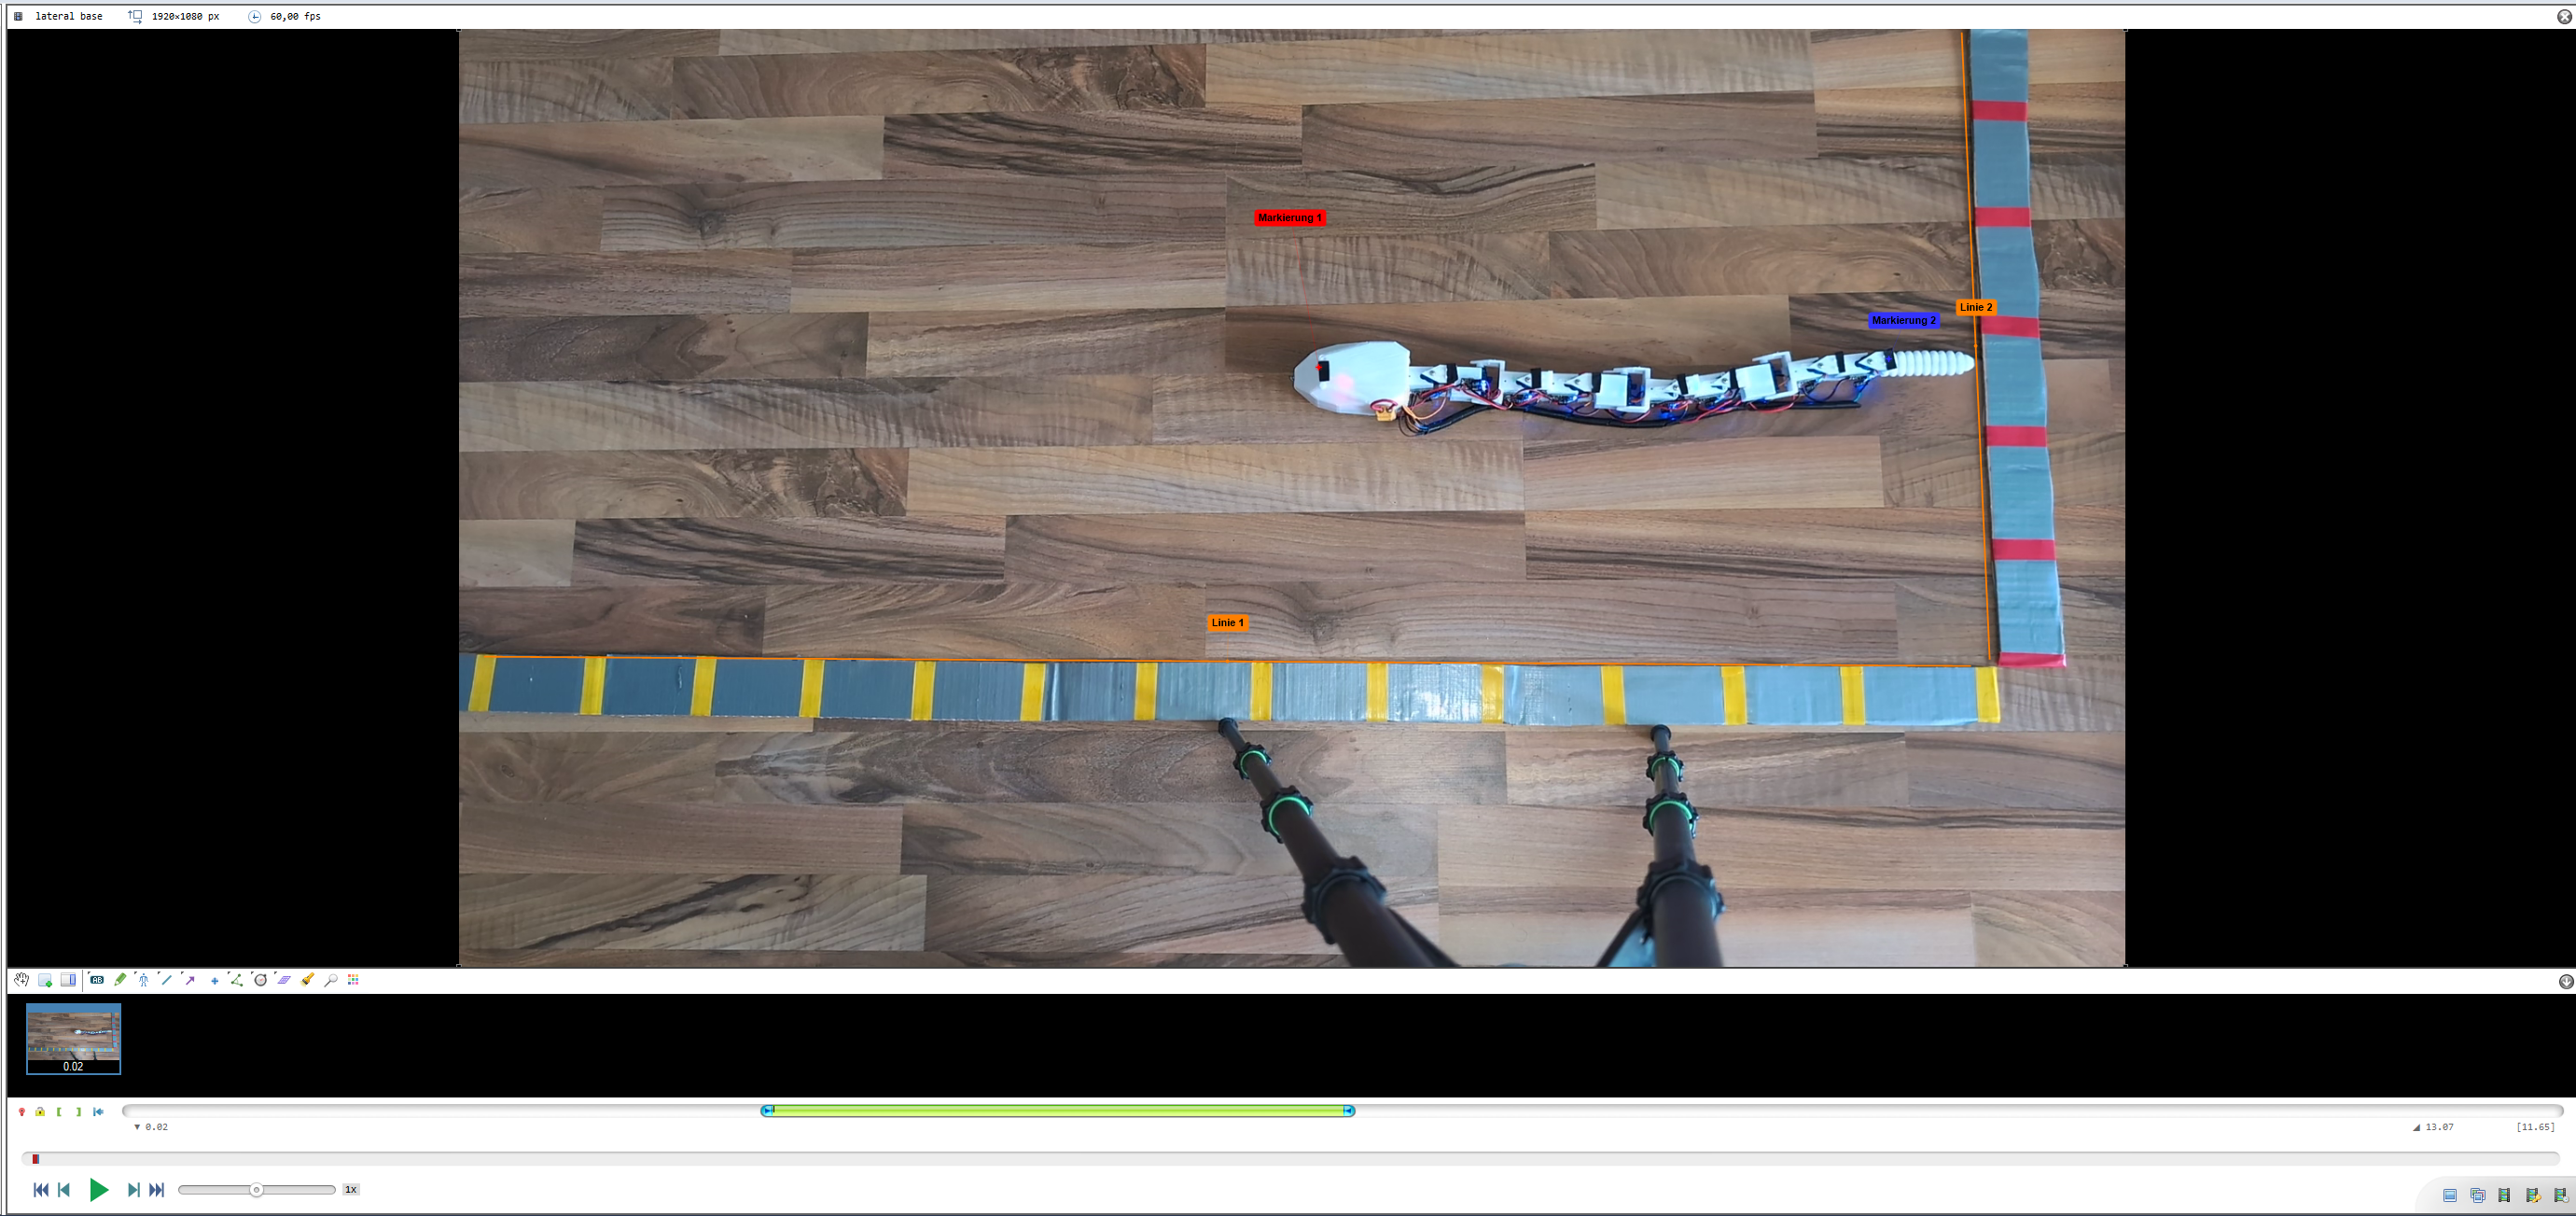
\includegraphics[width=0.8\textwidth]{media/kinovea.png}
\caption{Kinovea motion analysis app interface}
\label{fig:kinovea}
\end{figure}

%////////////////////////////////////////////

\section{Locomotion Performance Results}
This section presents a comprehensive analysis of the snake robot's locomotion capabilities based on systematic experimental trials. Multiple configurations were tested to evaluate performance metrics. Tracking data was collected using visual markers positioned at the head and tail segments, enabling quantitative analysis of the robot's movement trajectories under various conditions. The experiments were conducted on a standardized laminate wood surface to ensure consistent environmental conditions across all trials.

\subsection{Effect of Configuration on Locomotion}
The robot configuration significantly influenced locomotion movement patterns on the laminate wood surface. Analysis of the tracking data revealed distinct movement characteristics for each configuration. Each experiment was repeated at least three times to establish reliable patterns, which were observed with minimal deviations across trials.

\subsection{Locomotion Pattern Analysis}
Detailed analysis of the tracking data revealed distinct movement characteristics across different robot configurations and locomotion modes. By examining the trajectories of both head and tail segments, several consistent patterns emerged that provide insight into the complex dynamics of snake-like locomotion. The following analysis categorizes these observations into specific aspects of the robot's movement behavior, highlighting key factors that influence performance and stability during operation.

\subsubsection{Differential Weight Distribution Effects}
A key observation across all configurations was the influence of the robot's weight distribution. The snake-like robot has a noticeably heavier head than the tail, creating an uneven friction distribution along its body. This weight imbalance resulted in the head maintaining better grip on the surface while the lighter tail exhibited greater slippage, particularly in configurations without additional friction elements.

The head's greater mass resulted in more consistent contact with the surface and higher friction, allowing it to serve as an anchor point during movement. In contrast, the tail section frequently displayed observable slippage during propulsive movements, reducing locomotion efficiency and directional stability.

\subsubsection{Lateral Undulation Performance}
Lateral undulation showed distinct movement characteristics across the different configurations, as illustrated in Figure~\ref{fig:lateral_undulation_analysis}, which presents the horizontal and vertical head and tail positions based on the tracking data.

\begin{figure}[H]
    \centering
    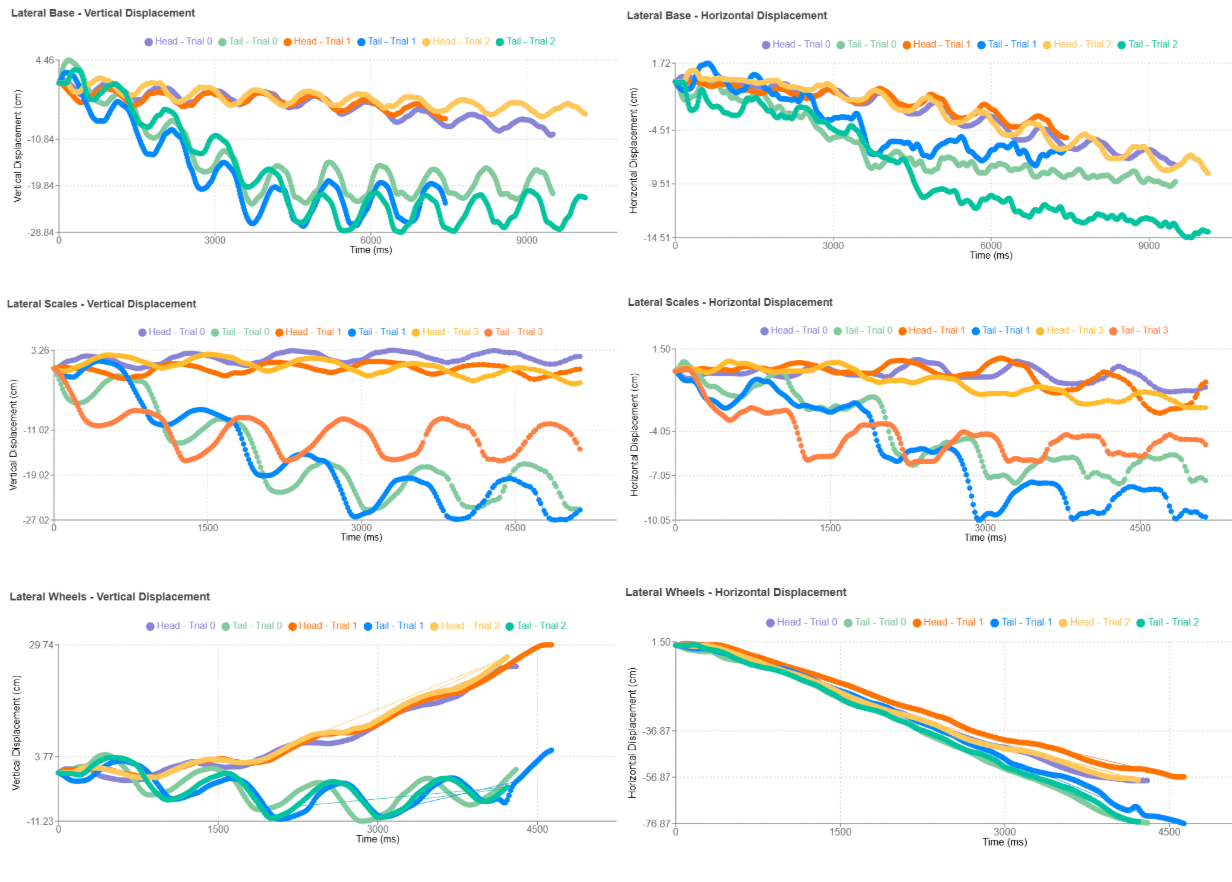
\includegraphics[width=1\textwidth]{media/lateral_undulation_trials.png}
    \caption{Head and tail trajectory patterns during lateral undulation for different configurations. Data generated from multiple trial runs using React visualization code.}
    \label{fig:lateral_undulation_analysis}
\end{figure}

With TPU scales attached, an interesting phenomenon was observed. The head remained in a relatively stationary position with minimal movement, functioning essentially as a pivot point. Meanwhile, the tail exhibited significant lateral slippage and movement. This differential between the stationary head and mobile tail resulted in the snake-like robot effectively rotating around its head position. The scales created such high friction at the head that it became anchored while the tail's movement generated rotational rather than forward motion.

The baseline configuration (without attachments) demonstrated a more distributed movement pattern. Without the additional friction element, the head also experienced slippage, though noticeably less compared to the tail. This allowed for more coordinated forward progression as both head and tail participated in the movement, albeit with the tail still showing greater lateral deviation due to its lighter weight. The reduced friction differential between head and tail in the baseline configuration resulted in less rotational movement and more linear progression.

The wheeled configuration demonstrated the most unified movement pattern during lateral undulation. The wheels created consistent rolling contact points that significantly reduced the slippage differential between head and tail. Both head and tail followed nearly parallel paths with minimal lateral deviation, resulting in a more direct forward progression. The wheels effectively compensated for the weight imbalance by providing uniform friction across the robot's body segments.

\subsubsection{Sidewinding Performance}
Sidewinding exhibited more complex movement patterns than initially anticipated. When the sidewinding algorithm was activated for forward progression, the robot moved sideways to the right. Interestingly, there was minimal difference in this behavior between the scaled and baseline configurations, suggesting that sidewinding is less dependent on surface friction compared to lateral undulation.

During this rightward sidewinding motion, the tail exhibited significantly more lateral movement than the head. This differential movement resulted in the tail generating a forward progression component while the head maintained a more stable position. The outcome was an arcing trajectory rather than the expected linear path.

When the sidewinding algorithm was executed in reverse, the robot moved to the left with a noticeably different pattern. In this direction, both head and tail showed more unified movement, resulting in a more consistent sideways displacement with less forward progression. This directional asymmetry suggested an underlying structural or algorithmic issue.

Further investigation of the robot's physical structure revealed a slight but significant design flaw. Along the chain of servo connections, a gradual tilt accumulates, resulting in the tail section having asymmetric ground contact. Specifically, one side of the tail maintains more consistent contact with the ground surface than the other. This structural asymmetry explains the different behavior patterns observed in rightward versus leftward sidewinding.

This asymmetric ground contact influenced the ground reaction forces experienced during sidewinding, creating the directional bias observed in the robot's movement. Figure~\ref{fig:sidewinding_analysis} illustrates these trajectory differences between rightward and leftward sidewinding patterns.

\begin{figure}[H]
    \centering
    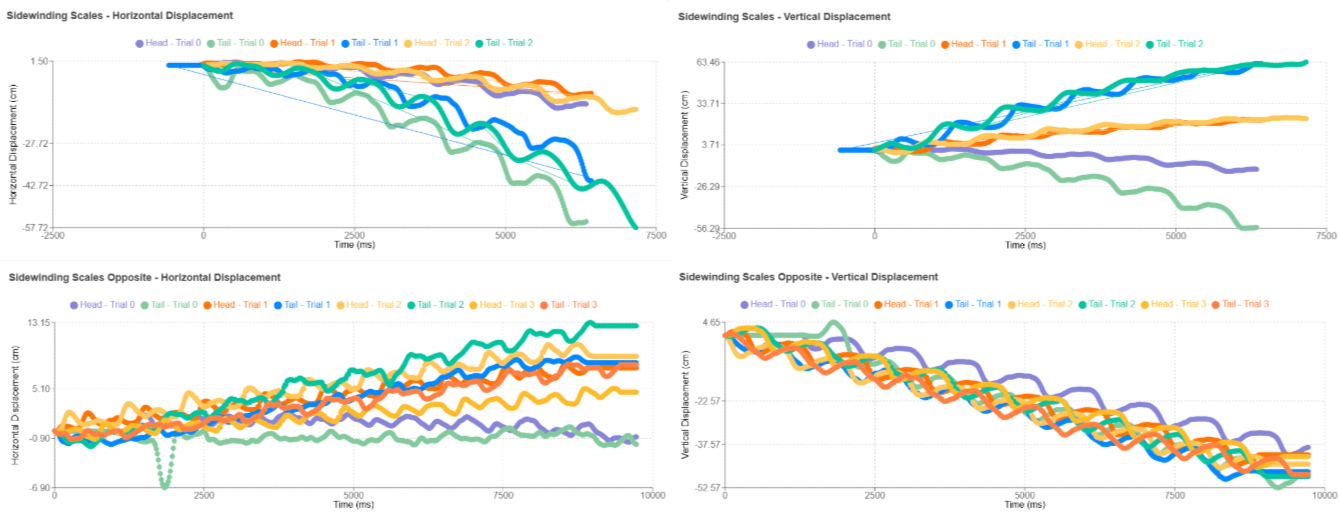
\includegraphics[width=1\textwidth]{media/sidewinding_direction_comparison.png}
    \caption{Head and tail trajectory paths during rightward and leftward sidewinding, showing asymmetric movement patterns due to structural tilt. Data compiled from multiple experimental trials and visualized using React-based graphing tools.}
    \label{fig:sidewinding_analysis}
\end{figure}

\subsubsection{Friction Enhancement and Movement Coordination}
A consistent finding across all locomotion patterns was that adding friction elements (either scales or wheels) unified the movement patterns between the head and tail sections. In both locomotion modes, slippage was observed more prominently in the baseline configuration without scales or wheels.

The addition of either scales or wheels served as a critical friction parameter that helped equalize the movement characteristics between the heavier, more stable head and the lighter, more slip-prone tail. This unification effect was particularly pronounced during directional changes, where the baseline configuration often showed the tail "whipping" or sliding unpredictably while the head maintained its intended path.

Repeated trials confirmed this pattern with minimal deviations, suggesting that friction enhancement is a fundamental factor in achieving coordinated snake-like locomotion on smooth surfaces like laminate flooring. The tracking data of head and tail positions on both vertical and horizontal axes consistently demonstrated that reducing the friction differential between body segments leads to more predictable and efficient movement patterns.

\section{Energy Consumption Analysis}
Power consumption was measured using the ACS712 current sensor integrated into the robot's power system. The ESP32 microcontroller recorded current measurements during operation, providing insights into the energy requirements of different locomotion strategies and configurations. Data was collected across multiple test runs for each locomotion mode and stored in CSV format for subsequent analysis.

\subsection{Experimental Setup and Data Collection}
For each locomotion mode, multiple experimental runs were conducted to ensure reproducibility and reliability of the measurements. Each experiment was time-synchronized, allowing for direct comparison between runs. The following locomotion modes were tested:

\begin{itemize}
    \item Idle Mode (robot powered but static)
    \item Lateral Undulation with Wheels
    \item Lateral Undulation with Scales
    \item Lateral Undulation Base (without additional locomotion aids)
    \item Sidewinding Base
    \item Sidewinding with Scales
\end{itemize}

Current measurements were recorded at a sampling rate of approximately 10 Hz, providing sufficient temporal resolution to capture transient effects during motion cycles.

\subsection{Idle Mode Current Draw}
The idle mode represents the baseline power consumption when the robot is powered but remaining stationary, with servos energized but not in motion.

\begin{figure}[H]
    \centering
    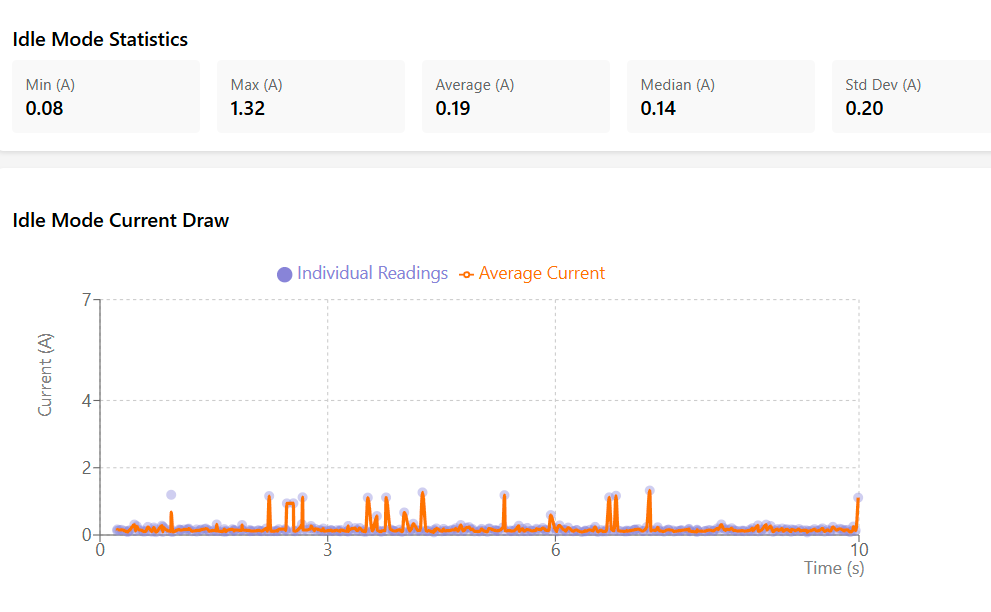
\includegraphics[width=12cm]{media/idle_mode_current.png}
    \caption{Current draw in idle mode across multiple experimental runs. The scatter plot shows individual measurements, while the solid line represents the average current.}
    \label{fig:idle_current}
\end{figure}

Analysis of the idle mode data revealed:
\begin{itemize}
    \item Current Range: 0.08--1.32 A
    \item Average Current: 0.19 A
    \item Median Current: 0.14 A
    \item Standard Deviation: 0.20 A
\end{itemize}

Even in idle mode, the current draw exhibited periodic fluctuations, likely due to the servos maintaining position against gravitational forces or small mechanical disturbances. These small peaks correspond to the servo motors drawing additional current to maintain their commanded positions.

\subsection{Lateral Undulation Current Analysis}
Three configurations of lateral undulation were tested: with wheels, with scales, and the base configuration. These configurations allow us to quantify the effect of different friction conditions on power consumption.

\begin{figure}[H]
    \centering
    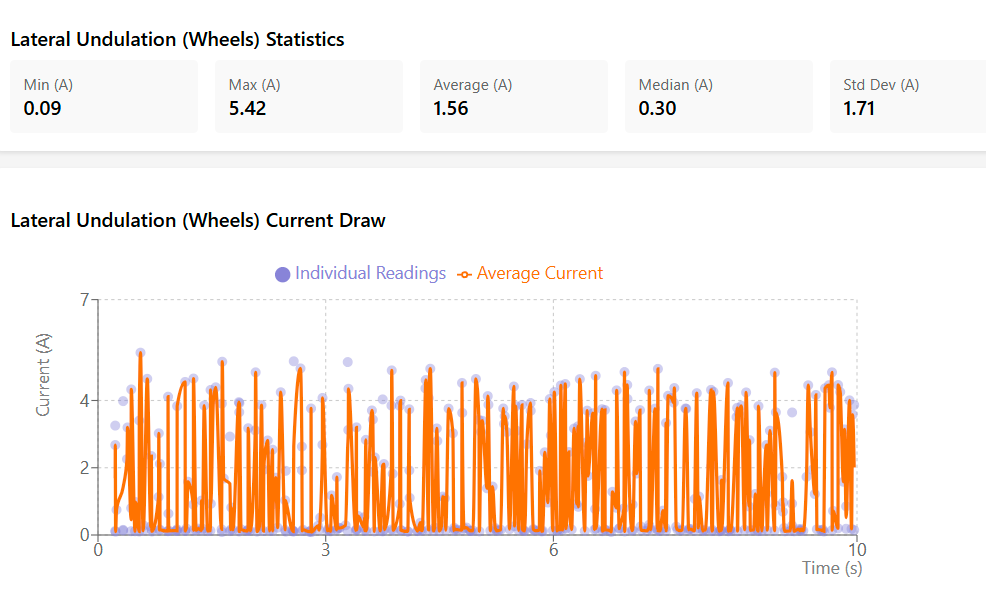
\includegraphics[width=12cm]{media/lateral_wheels_current.png}
    \caption{Current draw during lateral undulation with wheels. The scatter plot shows individual measurements across multiple runs, with the average current trend line overlaid.}
    \label{fig:lateral_wheels_current}
\end{figure}

\begin{figure}[H]
    \centering
    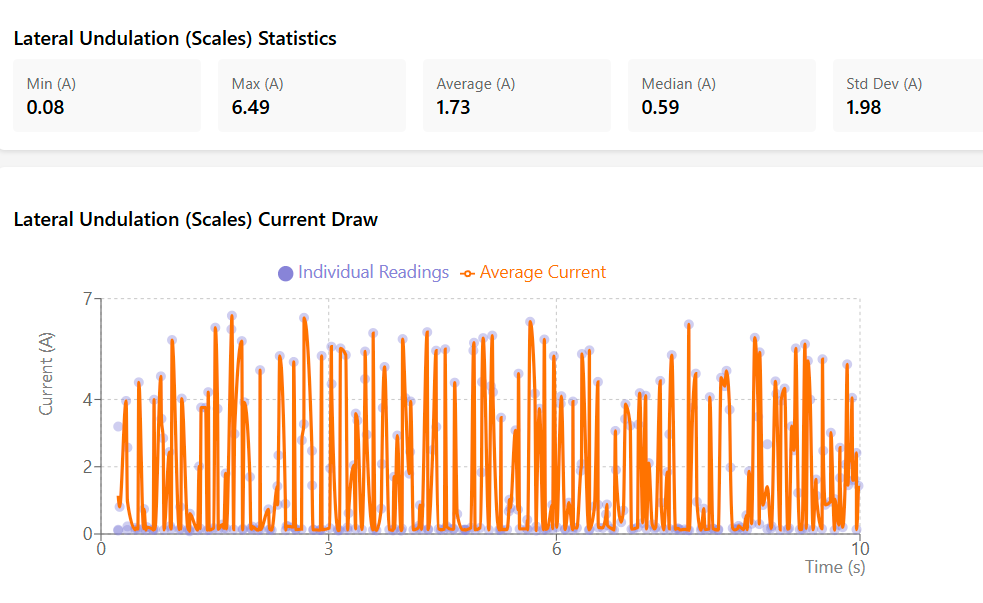
\includegraphics[width=12cm]{media/lateral_scales_current.png}
    \caption{Current draw during lateral undulation with scales. The scatter plot shows individual measurements across multiple runs, with the average current trend line overlaid.}
    \label{fig:lateral_scales_current}
\end{figure}

\begin{figure}[H]
    \centering
    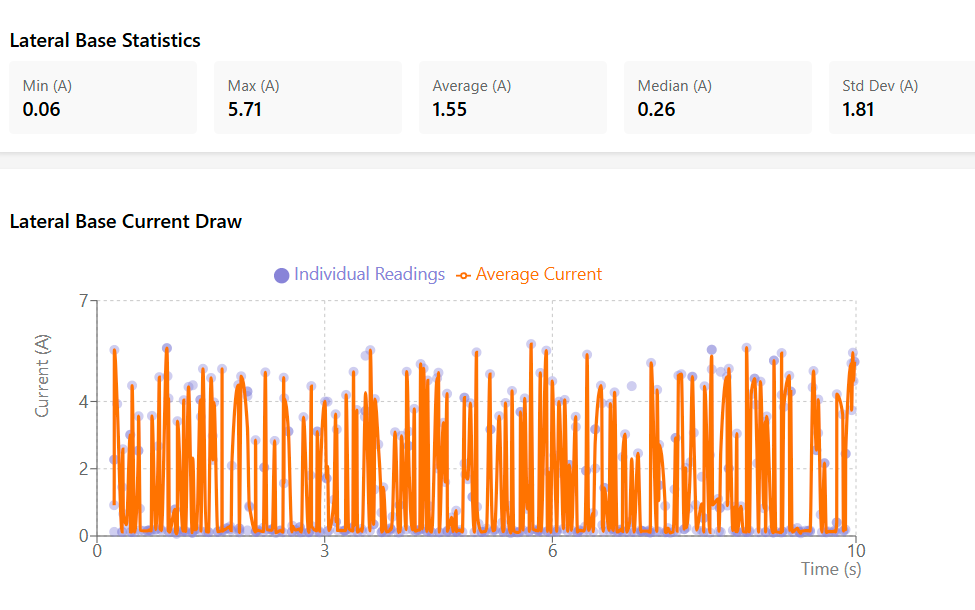
\includegraphics[width=12cm]{media/lateral_base_current.png}
    \caption{Current draw during lateral undulation in base configuration (without additional locomotion aids). The scatter plot shows individual measurements across multiple runs, with the average current trend line overlaid.}
    \label{fig:lateral_base_current}
\end{figure}

Key statistics for lateral undulation modes:

\begin{table}[H]
    \centering
    \adjustbox{max width=\textwidth}{
    \begin{tabular}{|l|c|c|c|c|}
        \hline
        \textbf{Configuration} & \textbf{Current Range (A)} & \textbf{Average (A)} & \textbf{Median (A)} & \textbf{Std Dev (A)}\\
        \hline
        Lateral Base & 0.06--5.71 & 1.55 & 0.26 & 1.81 \\
        \hline
        Lateral Undulation (Wheels) & 0.09--5.42 & 1.56 & 0.30 & 1.71 \\
        \hline
        Lateral Undulation (Scales) & 0.08--6.49 & 1.73 & 0.59 & 1.98 \\
        \hline
    \end{tabular}
    }
    \caption{Current consumption statistics across different lateral undulation configurations.}
    \label{tab:lateral_current_measurements}
\end{table}

The data reveals several important findings:
\begin{itemize}
    \item Lateral undulation with scales shows the highest average current draw (1.73 A) among the lateral locomotion modes, approximately 11\% higher than with wheels.
    \item The higher median value for scales configuration (0.59 A vs 0.30 A for wheels) indicates that scales consistently require more power throughout the motion cycle.
    \item All configurations exhibit significant current spikes, with the scales configuration reaching the highest peaks (up to 6.49 A), likely during direction changes or when overcoming static friction.
    \item The larger standard deviation in the scales configuration (1.98 A) suggests more variable power requirements depending on the phase of the motion pattern.
\end{itemize}

\subsection{Sidewinding Current Analysis}
Sidewinding represents a more complex three-dimensional motion pattern that involves coordinated vertical and horizontal movements. Two configurations were tested: the base sidewinding pattern and sidewinding with scales.

\begin{figure}[H]
    \centering
    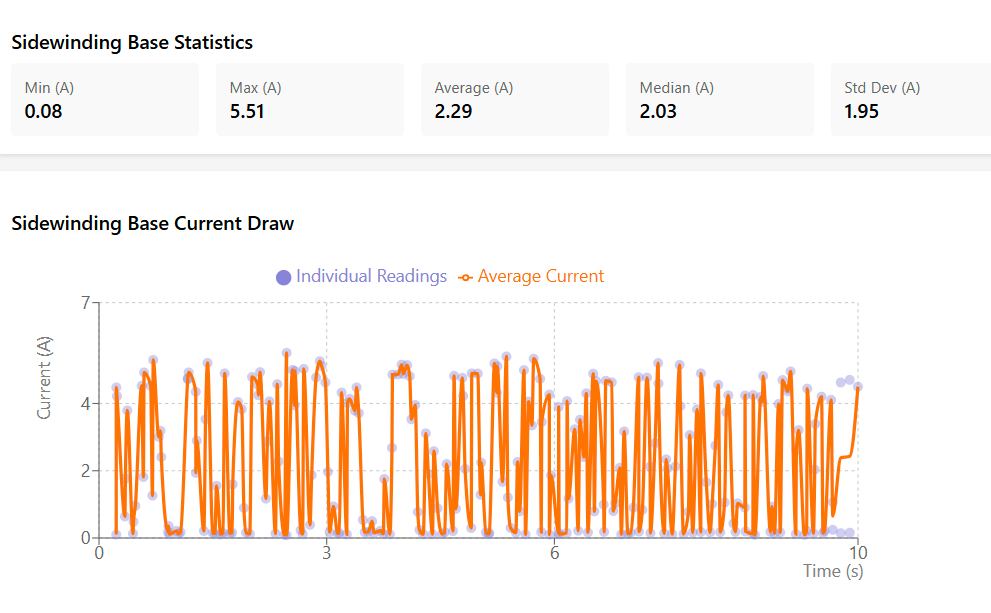
\includegraphics[width=12cm]{media/sidewinding_base_current.png}
    \caption{Current draw during sidewinding in base configuration. The scatter plot shows individual measurements across multiple runs, with the average current trend line overlaid.}
    \label{fig:sidewinding_base_current}
\end{figure}

\begin{figure}[H]
    \centering
    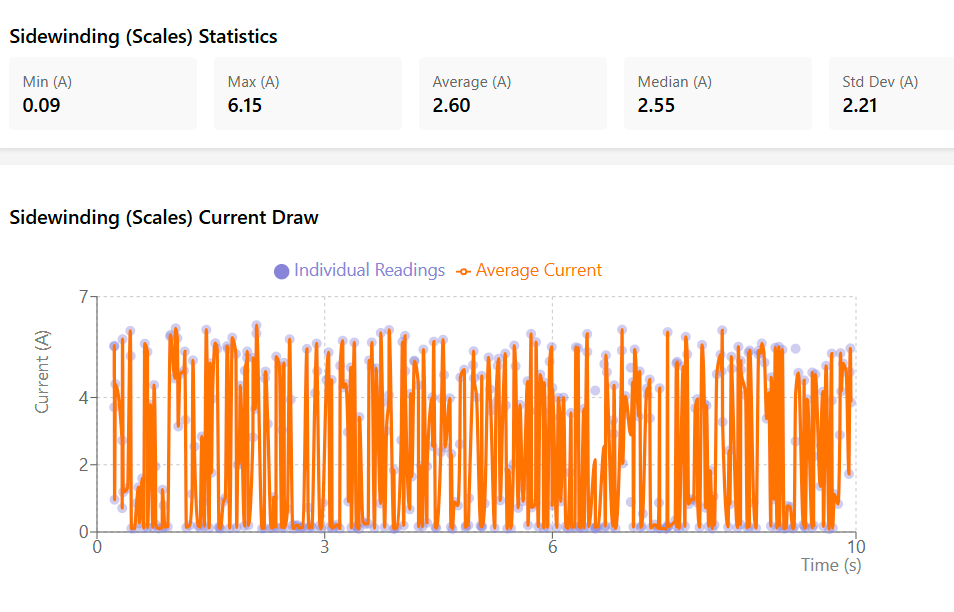
\includegraphics[width=12cm]{media/sidewinding_scales_current.png}
    \caption{Current draw during sidewinding with scales. The scatter plot shows individual measurements across multiple runs, with the average current trend line overlaid.}
    \label{fig:sidewinding_scales_current}
\end{figure}

Key statistics for sidewinding modes:

\begin{table}[H]
    \centering
    \adjustbox{max width=\textwidth}{
    \begin{tabular}{|l|c|c|c|c|}
        \hline
        \textbf{Configuration} & \textbf{Current Range (A)} & \textbf{Average (A)} & \textbf{Median (A)} & \textbf{Std Dev (A)}\\
        \hline
        Sidewinding Base & 0.08--5.51 & 2.29 & 2.03 & 1.95 \\
        \hline
        Sidewinding (Scales) & 0.09--6.15 & 2.60 & 2.55 & 2.21 \\
        \hline
    \end{tabular}
    }
    \caption{Current consumption statistics across different sidewinding configurations.}
    \label{tab:sidewinding_current_measurements}
\end{table}

Analysis of the sidewinding data reveals:
\begin{itemize}
    \item Both sidewinding configurations show significantly higher average and median current draw compared to lateral undulation modes, with sidewinding with scales consuming the most power overall (2.60 A average).
    \item The close values between median and average in sidewinding modes (especially with scales) indicates a more consistent power draw throughout the motion cycle, unlike the lateral modes which showed larger differences between median and average.
    \item Peak current values during sidewinding with scales reached 6.15 A, indicating substantial instantaneous power demands.
    \item The high standard deviation in both configurations (1.95-2.21 A) reflects the complex nature of the motion pattern, with significant variations in power requirements during different phases of the movement.
\end{itemize}

\subsection{Comparative Analysis of Locomotion Modes}
To better understand the relative energy efficiency of different locomotion strategies, a comparative analysis was performed across all tested configurations.

\begin{figure}[H]
    \centering
    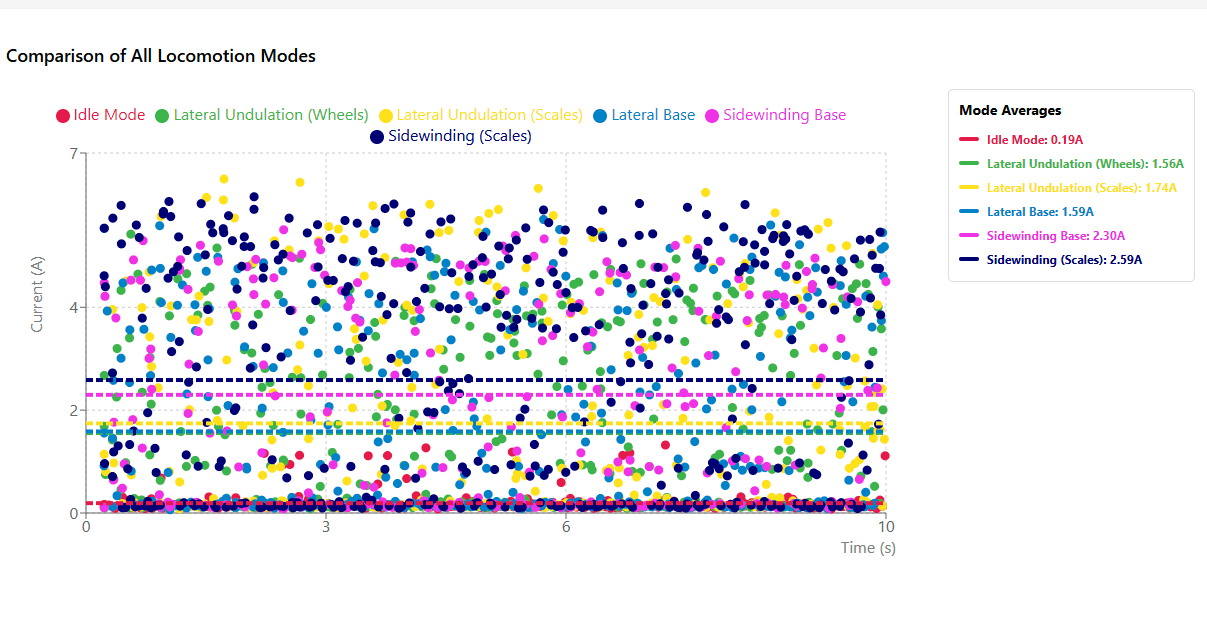
\includegraphics[width=12cm]{media/combined_current_comparison.png}
    \caption{Comparison of average current draw across all tested locomotion modes over a 10-second period. This visualization highlights the relative energy requirements of different motion strategies and configurations.}
    \label{fig:combined_current}
\end{figure}

\begin{table}[H]
    \centering
    \adjustbox{max width=\textwidth}{
    \begin{tabular}{|l|c|c|c|c|}
        \hline
        \textbf{Locomotion Mode} & \textbf{Current Range (A)} & \textbf{Average (A)} & \textbf{Median (A)} & \textbf{Std Dev (A)} \\
        \hline
        Idle Mode & 0.08--1.32 & 0.19 & 0.14 & 0.20 \\
        \hline
        Lateral Undulation (Wheels) & 0.09--5.42 & 1.56 & 0.30 & 1.71 \\
        \hline
        Lateral Undulation (Scales) & 0.08--6.49 & 1.73 & 0.59 & 1.98 \\
        \hline
        Lateral Base & 0.06--5.71 & 1.55 & 0.26 & 1.81 \\
        \hline
        Sidewinding Base & 0.08--5.51 & 2.29 & 2.03 & 1.95 \\
        \hline
        Sidewinding (Scales) & 0.09--6.15 & 2.60 & 2.55 & 2.21 \\
        \hline
    \end{tabular}
    }
    \caption{Comprehensive current consumption statistics across all locomotion modes.}
    \label{tab:current_measurements_complete}
\end{table}

Key comparative findings:
\begin{itemize}
    \item \textbf{Idle vs. Active Motion:} Any form of locomotion increases power consumption dramatically, with lateral undulation requiring approximately 8.2 times more power than idle mode (1.56-1.73 A vs. 0.19 A), and sidewinding requiring 12-13.7 times more power (2.29-2.60 A vs. 0.19 A).
    
    \item \textbf{Lateral Undulation Configurations:} The three lateral undulation configurations showed similar average current draw, with the scales configuration consuming only marginally more power (1.73 A) than the wheels (1.56 A) and base (1.55 A) configurations. However, the median values reveal that the scales configuration (0.59 A) maintains a higher baseline current throughout the motion cycle compared to the other configurations (0.26-0.30 A).
    
    \item \textbf{Sidewinding vs. Lateral Undulation:} Sidewinding motion patterns consume substantially more power than lateral undulation, with sidewinding with scales requiring approximately 50\% more energy than lateral undulation with scales (2.60 A vs. 1.73 A). This confirms that three-dimensional motion patterns involving both horizontal and vertical servo activation are significantly more power-intensive.
    
    \item \textbf{Effect of Scales:} The addition of scales consistently increased power consumption across both motion patterns, with a more pronounced effect in sidewinding (13.5\% increase) compared to lateral undulation (11\% increase). This highlights the impact of increased friction on energy requirements.
    
    \item \textbf{Peak Current Analysis:} All locomotion modes exhibited significant current spikes, with the highest peaks occurring in the lateral undulation with scales configuration (6.49 A). These spikes typically occurred during direction changes or when overcoming initial static friction. The high variability in current draw (as indicated by the large standard deviations) suggests opportunities for energy optimization by smoothing acceleration and deceleration profiles.
    
    \item \textbf{Consistency of Motion:} Sidewinding modes showed higher median values closer to their averages, indicating more consistent power draw throughout the motion cycle. In contrast, lateral undulation modes showed much lower median values compared to their averages, suggesting more intermittent high-current phases separated by lower-power periods.
\end{itemize}



%//////////////////
%//////////////////
%chapter 5
%//////////////////
%//////////////////
\chapter{Conclusion and Future Work}
\label{ch:conclusion}

This thesis has presented the development, implementation, and experimental evaluation of a neurobiologically inspired control system for a snake-like robot. The primary objectives were to (1) design and 3D-print a modular mechanical structure using Onshape, (2) integrate an ESP32 microcontroller with ten servo motors to achieve biomimetic locomotion, and (3) implement Central Pattern Generators (CPGs) in Arduino IDE to realize biologically-inspired movement patterns. The experimental results demonstrate that this approach can produce effective serpentine locomotion while maintaining relative simplicity in hardware and software design.

\section{Summary of Contributions}
\label{sec:contribution}

The main contribution of this work is the successful implementation of a biomimetic snake robot utilizing neurobiologically inspired control principles. A segment-based design was created in Onshape to emulate serpentine motion, enabling modular, repeatable segments that could be easily 3D-printed. The structure successfully balanced weight distribution concerns while providing sufficient robustness for extended testing. Three distinct configurations were developed and tested: a baseline version, one with TPU-printed passive scales representing a biomimetic approach, and one with wheels on each segment.

The hardware system was built around an ESP32 microcontroller serving as the central controller, interfacing with ten servo motors arranged in alternating horizontal and vertical orientations. This arrangement allowed for both lateral undulation and sidewinding motion patterns. The system was complemented with an ACS712 current sensor for power consumption analysis and a web interface for real-time control and data collection, enabling comprehensive performance evaluation during experimentation.

Two primary locomotion patterns were successfully implemented through CPG-inspired algorithms: lateral undulation and sidewinding. These algorithms generated sinusoidal wave patterns with configurable parameters including amplitude, frequency, and phase offset, closely mimicking biological snake movement. The implemented control system allowed for real-time parameter adjustment, enabling exploration of different movement characteristics and their impact on locomotion performance.

Extensive experimental testing was conducted using a structured grid environment and motion tracking software (Kinovea) to analyze the robot's movement patterns. The experiments yielded quantitative data on movement characteristics across different configurations and locomotion patterns, as well as detailed energy consumption measurements for all tested modes. This comprehensive analysis provided valuable insights into the complex relationships between mechanical configuration, control parameters, and resulting motion characteristics.

\section{Key Findings}
\label{sec:findings}

This section synthesizes the primary insights gained from the systematic evaluation of the snake robot's performance across multiple configurations and locomotion patterns.

\subsection{Locomotion Performance}
\label{subsec:loco_findings}

The experimental evaluation revealed that different robot configurations exhibited distinct movement characteristics that significantly impacted locomotion performance. The wheeled configuration provided the most uniform movement during lateral undulation, with minimal lateral deviation and the most direct forward progression. In contrast, the TPU scales configuration created such high friction at the head that it became anchored while the tail's movement generated rotational rather than forward motion.

A key observation across all configurations was the influence of the robot's uneven weight distribution. The snake-like robot had a noticeably heavier head than tail, creating an uneven friction distribution along its body. This weight imbalance resulted in the head maintaining better grip on the surface while the lighter tail exhibited greater slippage, particularly in configurations without additional friction elements. The head's greater mass resulted in more consistent contact with the surface and higher friction, allowing it to serve as an anchor point during movement. In contrast, the tail section frequently displayed observable slippage during propulsive movements, reducing locomotion efficiency and directional stability.

Sidewinding exhibited more complex movement patterns than initially anticipated. When the sidewinding algorithm was activated for forward progression, the robot moved sideways to the right with minimal difference in behavior between the scaled and baseline configurations. This suggested that sidewinding is less dependent on surface friction compared to lateral undulation. Interestingly, rightward sidewinding produced a slight arcing trajectory rather than the expected linear path, while leftward sidewinding showed more unified movement with consistent sideways displacement and less forward progression.

Further investigation revealed that a slight but significant structural asymmetry in the robot's design—specifically a gradual tilt accumulation along the servo chain—affected ground contact distribution and created directional bias during sidewinding movements. This asymmetric ground contact influenced the ground reaction forces experienced during sidewinding, explaining the directional bias observed in the robot's movement.

A consistent finding across all locomotion patterns was that adding friction elements (wheels) significantly unified the movement patterns between the head and tail sections. This unification effect was particularly pronounced during directional changes, where the baseline configuration often showed the tail "whipping" or sliding unpredictably while the head maintained its intended path.

\subsection{Energy Consumption}
\label{subsec:energy_findings}

The energy consumption analysis revealed significant differences between locomotion modes and configurations. Sidewinding movements required substantially more power than lateral undulation, with sidewinding with scales requiring approximately 50\% more energy than lateral undulation with scales (2.60 A vs. 1.73 A average current draw). This confirmed that three-dimensional motion patterns involving both horizontal and vertical servo activation are significantly more power-intensive.

The addition of scales consistently increased power consumption across both motion patterns, with a more pronounced effect in sidewinding (13.5\% increase) compared to lateral undulation (11\% increase). This highlighted the impact of increased friction on energy requirements. The three lateral undulation configurations showed similar average current draw, with the scales configuration consuming only marginally more power than the wheels and base configurations. However, the median values revealed that the scales configuration maintained a higher baseline current throughout the motion cycle compared to the other configurations.

\section{Limitations of the Current Implementation}
\label{sec:limitations}

Despite the promising results, several limitations were encountered during the experimental phase. One of the primary hardware constraints was the use of SG90 servos, which, while lightweight and compact, provided limited torque. This reduced the robot's ability to execute high-amplitude motions effectively and constrained its overall force output. Additionally, the system was powered by a single 18650 battery, which not only restricted the operating time but also limited the available power supply for the servos. As a result, maintaining consistent motion and torque output over extended periods proved challenging.

Another constraint arose from the ESP32's limited number of GPIO pins, which imposed a restriction on the number of servos that could be controlled simultaneously, limiting the potential for further expansion.Also the structural tilt along the robot body affected movement symmetry and ground contact distribution, creating the directional bias observed during sidewinding locomotion.

Beyond hardware limitations, several challenges were noted in software and control. The web-based control system, while functional, suffered from occasional WiFi interruptions, especially in environments with multiple overlapping networks, which impacted real-time responsiveness. Additionally, the ESP32 had to manage multiple tasks simultaneously, including web server communication, motion generation, and data logging. Under high processing loads, occasional slowdowns were observed, affecting the fluidity of motion execution.

Perhaps the most significant control limitation was the lack of direct feedback in the system. Operating in an open-loop configuration meant that there was no real-time positional or orientation feedback, making it difficult to dynamically adjust movements or compensate for external disturbances. This limited the robot's ability to adapt to changing environmental conditions or unexpected obstacles during locomotion.

\section{Future Improvements}
\label{sec:futureWork}
Based on the experimental results and performance analysis, several potential enhancements have been identified that could address the limitations observed in the current snake robot prototype. These improvements target specific aspects of the robot's design and functionality to enhance its locomotion capabilities.

\subsection{Enhanced Mechanical Design}
\label{subsec:mechanical_improvements}

Future iterations of the snake robot design should address the uneven weight distribution that causes differential friction between head and tail sections. A more balanced weight arrangement would promote more uniform movement and reduce unintended rotational tendencies during lateral undulation. This could be achieved through careful redistribution of electronic components or the strategic addition of counterweights in the tail section. Simultaneously, improvements in mechanical design should focus on eliminating the gradual tilt accumulation along the servo chain that created directional bias in sidewinding motion. More precise alignment mechanisms and structural reinforcement could mitigate this issue, ensuring more symmetrical movement in both directions.
Selective reinforcement at high-stress connection points could enhance longevity without significantly increasing weight.
Developing interchangeable friction elements would further enhance the robot's versatility across varied terrains. The current experimental results clearly demonstrated that different friction mechanisms (scales, wheels, or the baseline configuration) offer distinct advantages depending on the desired movement pattern and surface characteristics. A modular design allowing quick interchange between these configurations would enable rapid adaptation to changing environmental conditions and locomotion requirements.

\subsection{Power System Enhancements}
\label{subsec:power_improvements}

The energy consumption analysis highlighted several opportunities for power system improvements. Upgrading to higher capacity batteries or implementing a dual-battery system would extend operational runtime, particularly for power-intensive movements like sidewinding. The current consumption data indicates that sidewinding requires approximately 50\% more energy than lateral undulation, suggesting that power capacity is a critical factor for robots intended to utilize this movement pattern extensively.

Replacing the SG90 servos with higher-torque, more energy-efficient alternatives would improve motion capability while potentially reducing peak current demands through better mechanical efficiency. More powerful servos would also enable more reliable execution of high-amplitude movements, potentially improving locomotion effectiveness on challenging terrains. The current spikes observed during motion transitions suggest that implementing intelligent power management that dynamically adjusts servo parameters based on battery state and motion requirements could significantly extend operational duration.
Developing smoother acceleration and deceleration profiles could reduce the current spikes observed during transitions, potentially lowering peak power demands and improving overall efficiency. 

\subsection{Low-Latency Control with ESP-NOW}
\label{subsec:esp_now_control}

While the web interface provided a functional control mechanism for the snake robot, it introduced noticeable latency due to the HTTP request processing and potential WiFi network congestion. Future iterations of the system could benefit significantly from implementing ESP-NOW, a peer-to-peer protocol developed by Espressif that offers lower latency and reduced power consumption compared to traditional WiFi connections.

ESP-NOW would enable the development of a dedicated handheld controller using another ESP32 board, creating a direct communication channel with the snake robot. This approach offers several key advantages: response times could be reduced from hundreds of milliseconds to less than 10ms, providing near real-time control that would allow for more precise manipulation of the robot's movements. The protocol's lightweight nature would reduce the processing overhead on the ESP32 controller, potentially freeing computational resources for more complex locomotion algorithms or sensor processing.
Additionally, ESP-NOW's simplified connection mechanism eliminates the need for the snake robot to maintain an access point and web server, reducing power consumption and extending battery life. The protocol also offers greater operational range compared to the current web interface approach, potentially allowing control from distances of up to 400 meters in open areas. Implementation would require developing a custom controller with joysticks, buttons, and potentially a small display to provide feedback on robot parameters such as battery status and current locomotion mode.
For educational and research applications, this system could be extended to allow seamless switching between autonomous operation (utilizing the CPG algorithms) and direct operator control.


\subsection{Advanced Control Algorithms}
\label{subsec:control_improvements}

The open-loop control system used in the current implementation showed promising results but lacked the ability to adapt to changing conditions or compensate for structural asymmetries. Integrating sensors such as IMUs (Inertial Measurement Units) would enable closed-loop control, allowing the robot to adapt its movement based on real-time feedback about its position, orientation, and movement characteristics. This feedback could be used to dynamically adjust CPG parameters to maintain desired movement trajectories despite environmental disturbances or mechanical asymmetries.

Machine learning algorithms could be implemented to dynamically adjust CPG parameters (frequency, amplitude, phase offset) based on environmental conditions and performance feedback. This adaptive approach could optimize locomotion efficiency across different terrains by automatically selecting the most effective parameter combinations based on sensed conditions and movement outcomes. The system could learn from experience, progressively refining its parameter selection to improve performance over time.

\subsection{Extended Applications}
\label{subsec:applications}

The modular snake-like robot design developed in this thesis has potential applications beyond the experimental context. With further development, the system could be adapted for confined-space exploration and search and rescue operations, leveraging its ability to navigate narrow passages inaccessible to traditional robots. The snake's flexible body configuration and ability to execute three-dimensional movement patterns make it well-suited for traversing complex environments with limited clearance.

The design could also be adapted for pipeline or structural inspection tasks by integrating appropriate sensors and enhancing the robot's ability to navigate vertical surfaces. The potential for sidewinding movement on inclined surfaces, combined with the robot's elongated body, makes it a promising platform for industrial inspection applications where access is limited and maneuverability is essential.

In educational contexts, simplified versions of the system could serve as platforms for teaching principles of biomimetic robotics, control systems, and 3D design and fabrication. The accessible hardware platform (ESP32) and software environment (Arduino IDE) make the system approachable for educational purposes, while the clear relationship between biological principles and robotic implementation provides valuable learning opportunities.

Exploring the potential for multiple snake robots to coordinate their movements could lead to novel applications in distributed sensing or collaborative manipulation tasks. For example, a group of snake robots could form temporary structures or cooperatively transport objects by leveraging their flexible bodies and varied movement capabilities.

\section{Concluding Remarks}
\label{sec:concludingRemarks}

This thesis has demonstrated that a neurobiologically inspired approach to snake robot design and control can produce effective biomimetic locomotion using accessible hardware and software platforms. The detailed experimental analysis has provided valuable insights into the complex relationships between mechanical configuration, control parameters, and movement characteristics, highlighting both the potential and challenges of snake-like robotic systems.

The findings underscore the importance of considering weight distribution, ground contact dynamics, and energy efficiency in biomimetic robot design. The significant differences observed between locomotion patterns and configurations emphasize the need for adaptive, context-sensitive control approaches that can leverage the unique advantages of different movement strategies. The energy consumption analysis revealed important trade-offs between movement capability and operational duration, providing a foundation for future optimization efforts.

While the current implementation has certain limitations in terms of hardware capabilities and control sophistication, it provides a solid foundation for future research and development. The modular design approach, combined with the accessible ESP32 platform and Arduino IDE environment, creates a flexible experimental platform that can evolve to address increasingly complex challenges in biomimetic robotics.

As this field continues to advance, the integration of more sophisticated sensing, adaptive control algorithms, and optimized mechanical designs will push the boundaries of what snake-like robots can achieve. These systems hold significant promise for applications ranging from search and rescue operations to industrial inspection where their unique locomotion capabilities provide advantages over traditional wheeled or legged robots.

The neurobiological principles that inspired this work remain a rich source of insights for future robotic systems, highlighting how the elegant solutions evolved in biological organisms can inform the development of more adaptive, efficient, and versatile robotic technologies. By continuing to draw inspiration from nature while leveraging advances in materials, sensors, and computational capabilities, we can develop increasingly sophisticated biomimetic robots that combine the best aspects of biological and engineered systems.


% Appendices 
\appendix
%//////////////////////////////////////
%//////////////////////////////////////
%//////////////////////////////////////
%//////////////////////////////////////
%//////////////////////////////////////
\chapter{Hardware Specifications}
\section{Mechanical Design}
\subsection{3D Printed Components}

The snake robot is constructed from a variety of meticulously designed 3D-printed components, each engineered for structural integrity, modularity, and optimal functionality. All parts are 3D printed using PETG, PLA, PLA+, and TPU filaments, with tailored print settings that balance detail, strength, and weight.

\FloatBarrier
\subsubsection{Head Assembly}
The head assembly is divided into two primary sections: the \textbf{top-head} and the \textbf{bottom-head}. Together, they not only secure critical sensors and electronics but also enhance the aesthetic and structural characteristics of the robot. Key attributes include:
\begin{itemize}
    \item \textbf{Material:} PETG
    \item \textbf{Print Settings:} 0.2\,mm layer height with 30\% gyroid infill
    \item \textbf{Design Features:}
    \begin{itemize}
        \item Reinforced mounting slots for secure sensor and electronics placement
        \item A structured surface that blends visual appeal with mechanical strength
    \end{itemize}
\end{itemize}

\begin{figure}[H]
\centering
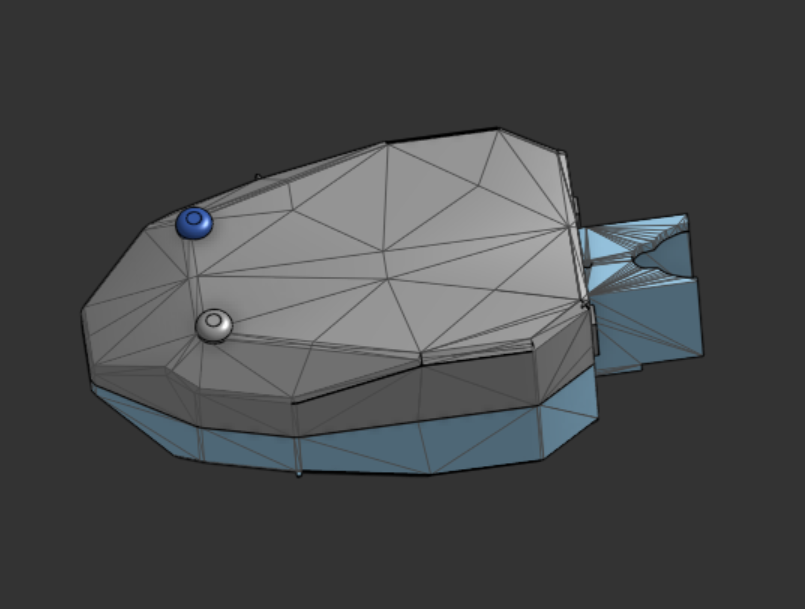
\includegraphics[width=0.5\textwidth]{media/Head.png}
\caption{Complete head assembly}
\par\vspace{4 mm}
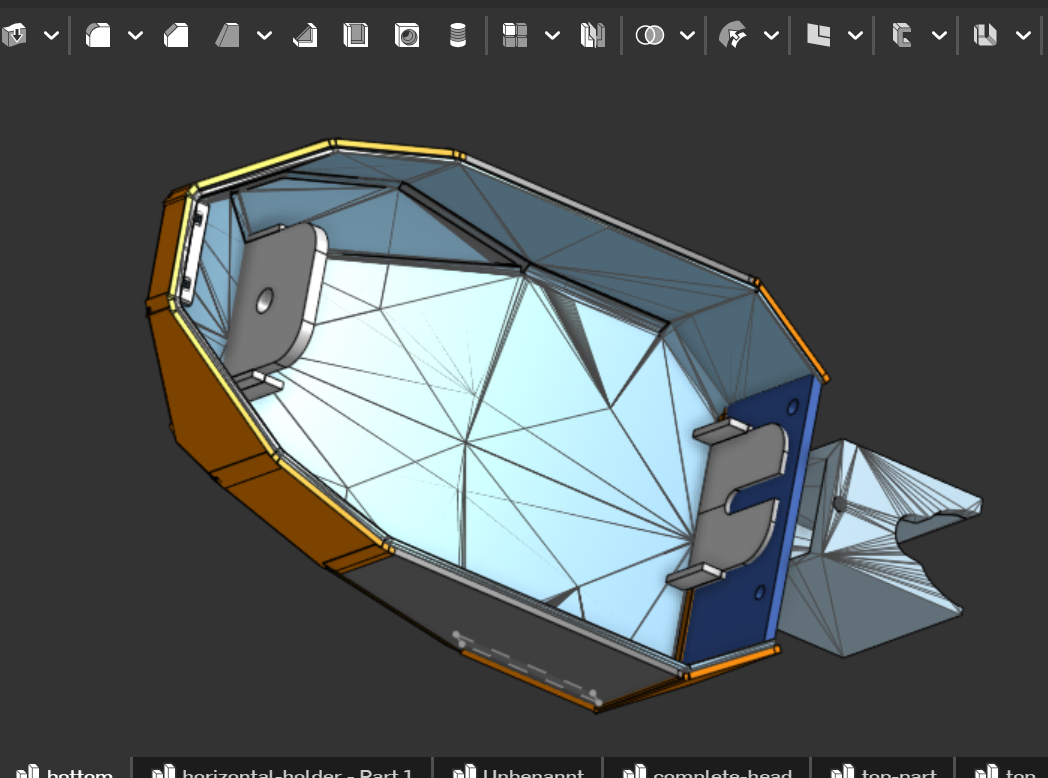
\includegraphics[width=0.5\textwidth]{media/Bottom-Head.png}
\caption{Bottom head assembly}
\par\vspace{4 mm}
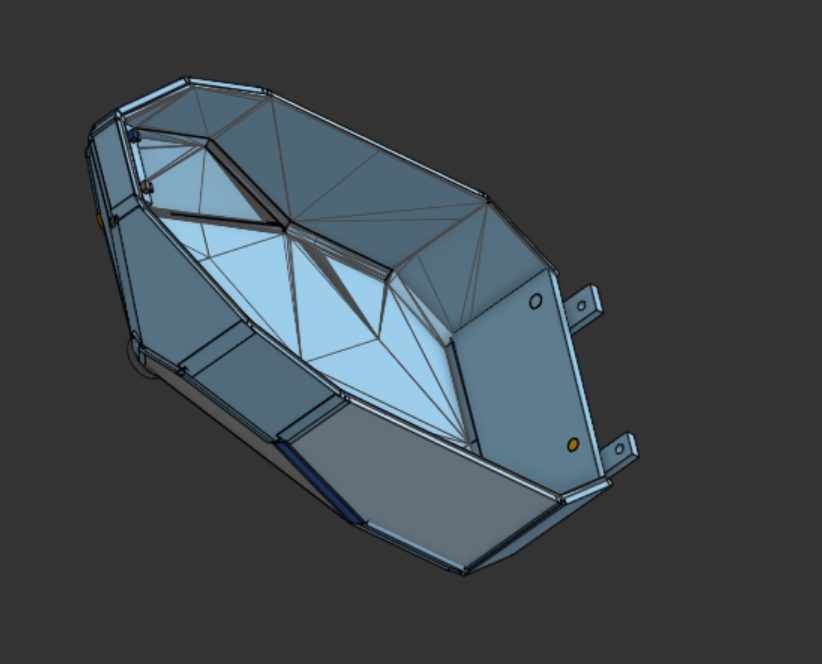
\includegraphics[width=0.5\textwidth]{media/top-head.png}
\caption{Combined view of the top and bottom head sections}
\end{figure}

\FloatBarrier
\subsubsection{Tail Structure}
The tail serves as a critical connector between the main body and the rear stabilizers, enabling controlled movement. Its design emphasizes both functionality and ease of integration:
\begin{itemize}
    \item \textbf{Material:} PETG
    \item \textbf{Print Settings:} 0.2\,mm layer height with 30\% infill
    \item \textbf{Key Features:}
    \begin{itemize}
        \item Reinforced mounting points designed for servo attachment
        \item Aesthetical rattlesnake tail design
    \end{itemize}
\end{itemize}

\begin{figure}[H]
\centering
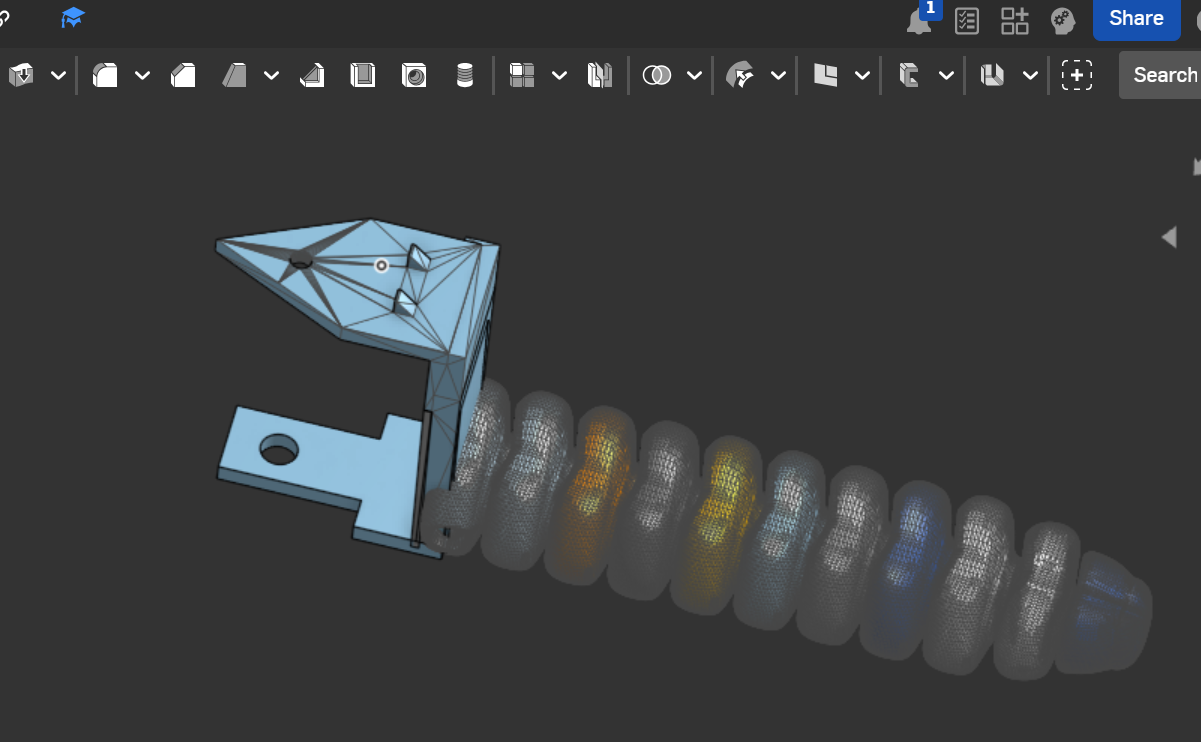
\includegraphics[width=0.5\textwidth]{media/Tail-part.png}
\caption{Tail structure assembly}
\end{figure}

\FloatBarrier
\subsubsection{Scales for Friction Optimization}
To enhance traction and optimize friction during movement, the robot incorporates an array of overlapping scales. These components are engineered for both flexibility and durability:
\begin{itemize}
    \item \textbf{Material:} TPU
    \item \textbf{Print Settings:} 0.1\,mm layer height to capture fine details
    \item \textbf{Design Characteristics:}
    \begin{itemize}
        \item Lightweight construction without compromising strength
        \item Flexible attachment points to adapt during motion
        \item A textured surface optimized for improved traction
    \end{itemize}
\end{itemize}

\begin{figure}[H]
\centering
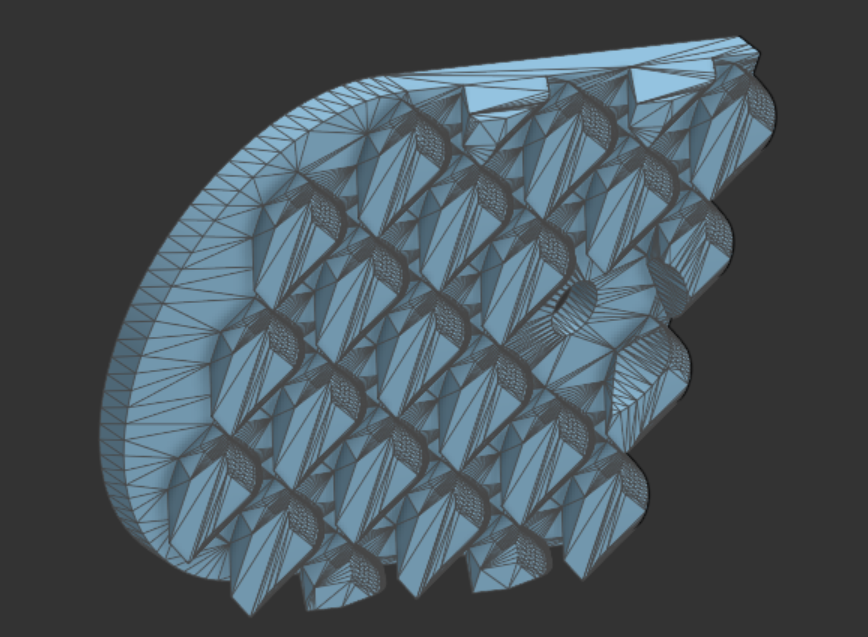
\includegraphics[width=0.5\textwidth]{media/scales.png}
\caption{3D printed scales for enhanced movement}
\end{figure}

\FloatBarrier
\subsubsection{Servo Holders}
Servo holders are integral to the robot's actuation system, providing secure and versatile mounting options for the servos. Two configurations are used:
\begin{itemize}
    \item \textbf{Material:} PETG
    \item \textbf{Print Settings:} 0.2\,mm layer height with 30\% infill for maximum strength
    \item \textbf{Features:}
    \begin{itemize}
        \item A snap-fit design that simplifies installation and removal
        \item Screw holes ensuring a stable and secure mounting
    \end{itemize}
\end{itemize}

\begin{figure}[H]
\centering
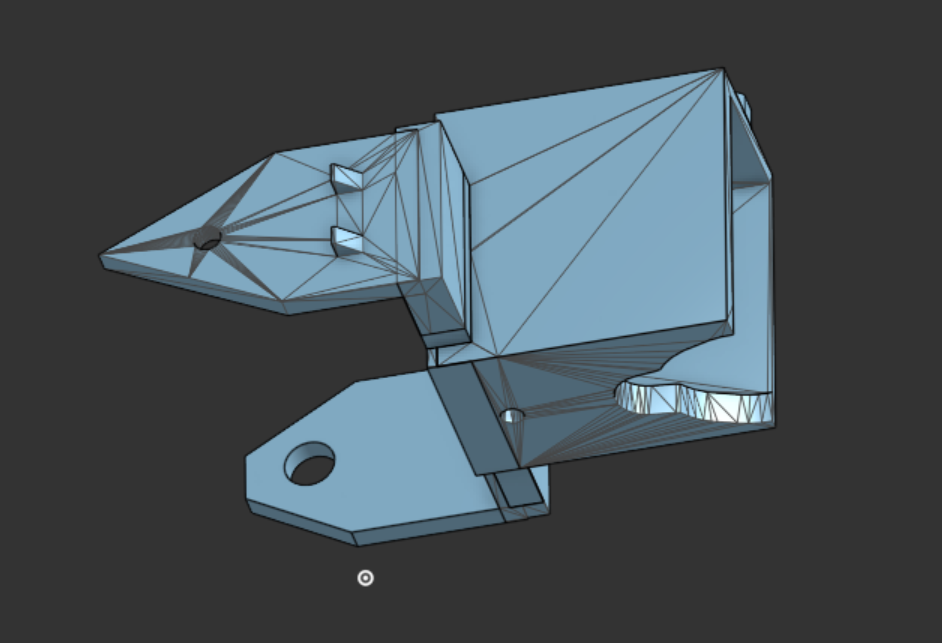
\includegraphics[width=0.5\textwidth]{media/Vertical-holder.png}
\caption{Vertical servo holder}
\par\vspace{4 mm}
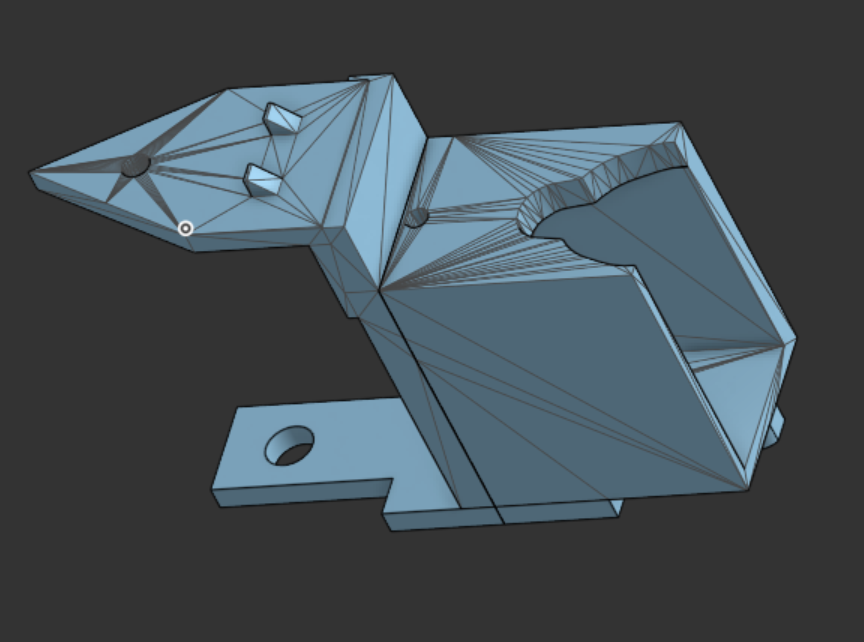
\includegraphics[width=0.5\textwidth]{media/Horizontal-holder.png}
\caption{Horizontal servo holder}
\end{figure}

\FloatBarrier
\subsubsection{Wheelbase, Wheel, and Tire}
A robust locomotion system is realized through the integration of a wheelbase, wheels, and tires:
\begin{itemize}
    \item \textbf{Wheelbase:} Positioned beneath the main body segments, each unit supports two small wheels to stabilize movement.
\end{itemize}

\begin{figure}[H]
\centering
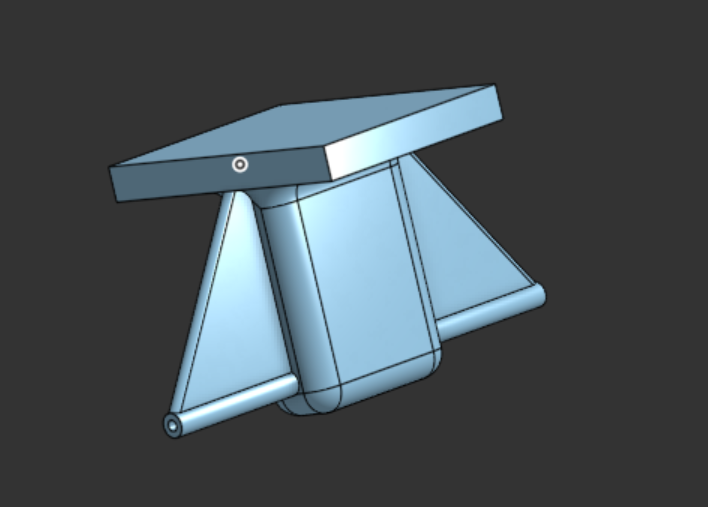
\includegraphics[width=0.5\textwidth]{media/Wheelbase.png}
\caption{Wheelbase assembly}
\end{figure}

\begin{itemize}
    \item \textbf{Wheel:} Engineered for smooth rotation and effective support.
\end{itemize}
\begin{itemize}
    \item \textbf{Tire:} Designed to provide optimal traction and cushioning during locomotion.
\end{itemize}

\begin{figure}[H]
\centering
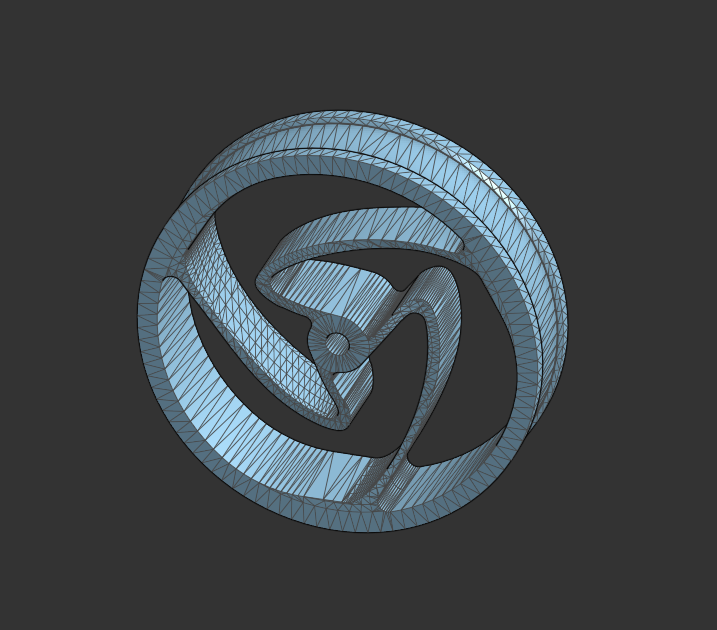
\includegraphics[width=0.5\textwidth]{media/Wheel.png}
\caption{Wheel component}
\end{figure}
\begin{figure}[H]
\centering
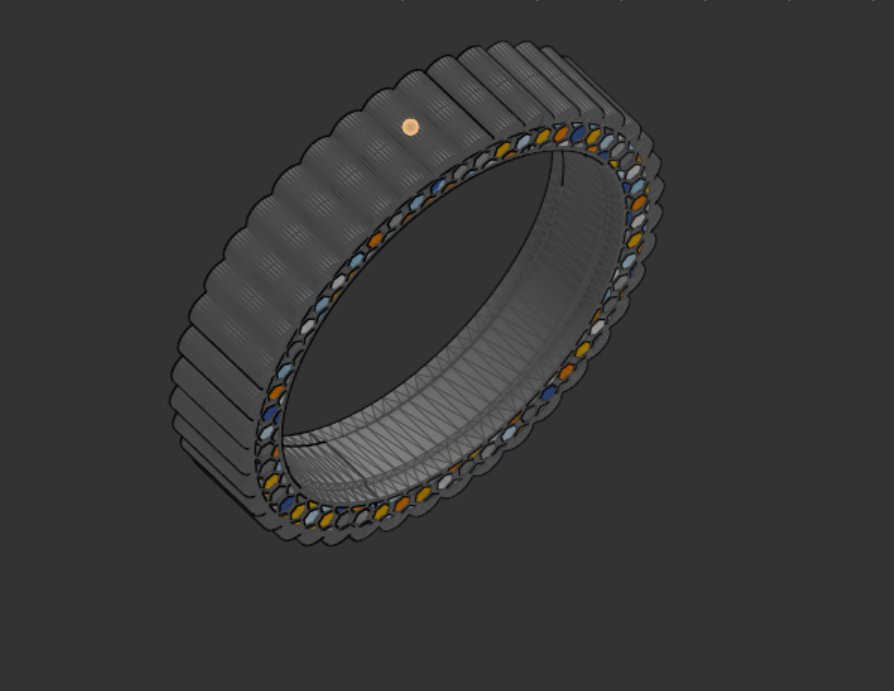
\includegraphics[width=0.5\textwidth]{media/Tire.png}
\caption{Tire component}
\end{figure}

\section{Electronic Components}
\subsection{Microcontroller Specifications}
\begin{itemize}
\item ESP32-WROOM-32 Development Board:
\begin{itemize}
\item Dual-core Xtensa LX6 microprocessor
\item Operating frequency up to 240 MHz
\item 520 KB SRAM
\item 4 MB Flash memory
\item Integrated WiFi 802.11 b/g/n
\item Bluetooth 4.2 support
\item Operating voltage: 3.3V
\item 34x programmable GPIO pins
\end{itemize}
\end{itemize}
\subsection{Servo Motor Details}
\begin{table}[H]
\centering
\begin{tabular}{|l|l|}
\hline
\textbf{Parameter} & \textbf{Value} \\
\hline
Model & SG90 \\
Operating Voltage & 4.8\,V -- 6.0\,V \\
Stall Torque (4.8\,V) & $\approx$1.5\,kg$\cdot$cm \\
Operating Speed (4.8\,V) & 0.12\,sec/60$^{\circ}$ \\
Operating Angle & 180$^{\circ}\,\pm\,5^{\circ}$ \\
Pulse Width Range & 500--2400\,$\mu$s \\
Direction & Bi-directional (CW/CCW) \\
Gear Type & Plastic Gears \\
Weight & 9\,g \\
Dimensions & 22.8\,$\times$\,12.2\,$\times$\,28.5\,mm \\
\hline
\end{tabular}
\caption{SG90 servo motor specifications.}
\end{table}

\subsection{Power System}
\begin{itemize}
    \item \textbf{Battery:}
    \begin{itemize}
        \item \textit{Type}: Single 18650 Li-ion cell
        \item \textit{Voltage}: 3.7\,V nominal (4.2\,V max)
        \item \textit{Capacity}: (varies by cell, e.g., 2200\,mAh)
        \item \textit{Weight}: $\approx$45\,g (typical for 18650)
    \end{itemize}

    \item \textbf{Power Distribution:}
    \begin{itemize}
        \item Buck converter regulating output to 5\,V for servos and controller
        \item Simple on/off switch for power control
        \item Note: The user must monitor battery voltage externally (no built-in protection circuit)
    \end{itemize}
\end{itemize}

 
%//////////////////////////////////////
%//////////////////////////////////////
%//////////////////////////////////////
%//////////////////////////////////////
%//////////////////////////////////////

\chapter{Snake Robot Software Implementation}

\section{System Architecture}
The snake robot's control software is implemented on an ESP32 microcontroller using the Arduino IDE. The system architecture comprises several integrated components:

\begin{enumerate}
    \item \textbf{Motion Control System}: Implements two primary locomotion patterns (lateral undulation and sidewinding)
    \item \textbf{Servo Motor Management}: Controls 10 servo motors in a specific layout (7 horizontal, 3 vertical)
    \item \textbf{Web-Based Interface}: Provides remote control through a WiFi access point and user-friendly HTML interface
    \item \textbf{Current Monitoring}: Measures power consumption with ACS712 current sensor
    \item \textbf{Data Logging System}: Records current measurements to the ESP32's SPIFFS filesystem
    \item \textbf{Diagnostic Tool}: Includes servo-testing.
\end{enumerate}

\section{Hardware Configuration}

\subsection{Servo Configuration}
The robot consists of 10 servo motors with a specific arrangement of horizontal and vertical actuators:

\begin{minted}[frame=single, linenos, breaklines, breakanywhere, fontsize=\footnotesize]{c++}
// Servo configuration
const int NUM_SERVOS = 10;
const int NUM_HORIZONTAL = 7;  // Number of horizontal servos
const int servoLayout[NUM_SERVOS] = {1, 0, 1, 1, 0, 1, 1, 0, 1, 1}; // 1=horizontal, 0=vertical
const int servoPins[NUM_SERVOS] = {23, 22, 2, 4, 16, 17, 5, 18, 19, 21};
\end{minted}

\subsection{Sensor Configuration}
The current sensing is implemented using an ACS712 current sensor:

\begin{minted}[frame=single, linenos, breaklines, breakanywhere]{c++}
const int analogPin = 34;
ACS712 sensor(analogPin, 3.3, 4095, 100.0); // pin, voltage, ADC max, mV/A sensitivity
\end{minted}

\section{Locomotion Control System}

\subsection{Motion Parameters}
The locomotion patterns are controlled by the following parameters:

\begin{minted}[frame=single, linenos,breaklines, breakanywhere, fontsize=\footnotesize]{c++}
// Locomotion parameters
float amplitude = 30.0;           // Degrees
float frequency = 1.0;            // Hz
float phaseOffset = 60.0;         // Degrees
float verticalAmplitude = 20.0;   // For sidewinding (degrees)
float verticalPhaseOffset = 90.0; // 90 degrees offset for sidewinding
float centerPosition = 90.0;      // Degrees
\end{minted}

\subsection{Lateral Undulation}
The lateral undulation algorithm generates a sinusoidal wave that propagates through the horizontal servos:

\begin{minted}[frame=single, linenos, breaklines, breakanywhere]{c++}
void updateServosLateralUndulation() {
  float timeScale = millis() * 0.001 * frequency * 2 * PI;
  int horizontalIndex = 0;
  
  for (int i = 0; i < NUM_SERVOS; i++) {
    if (servoLayout[i] == 1) {  // Horizontal servos
      float segmentPhase;
      
      if (forwardDirection) {
        // For forward motion, reverse the phase progression
        segmentPhase = (NUM_HORIZONTAL - 1 - horizontalIndex) * radians(phaseOffset);
      } else {
        // For backward motion, use the original phase progression
        segmentPhase = horizontalIndex * radians(phaseOffset);
      }
      
      // Calculate servo angle with full amplitude
      float angle = centerPosition + amplitude * sin(timeScale + segmentPhase);
      
      servos[i].write(angle);
      horizontalIndex++;
    } else {  // Vertical servos remain centered
      servos[i].write(centerPosition);
    }
  }
}
\end{minted}

\subsection{Sidewinding Motion}
The sidewinding algorithm creates coordinated waves in both horizontal and vertical planes:

\begin{minted}[frame=single, linenos,breaklines, breakanywhere]{c++}
void updateServosSidewinding() {
  float timeScale = millis() * 0.001 * frequency * 2 * PI;
  int horizontalIndex = 0;
  int verticalIndex = 0;

  for (int i = 0; i < NUM_SERVOS; i++) {
    if (servoLayout[i] == 1) {  // Horizontal servos
      float phase = forwardDirection ? 
        radians((NUM_HORIZONTAL - 1 - horizontalIndex) * phaseOffset) : 
        radians(horizontalIndex * phaseOffset);
      
      float angle = centerPosition + amplitude * sin(timeScale + phase);
      servos[i].write(angle);
      horizontalIndex++;
    } else {  // Vertical servos
      float basePhase = verticalIndex * phaseOffset + verticalPhaseOffset;
      float phase = forwardDirection ? 
        radians((NUM_SERVOS - NUM_HORIZONTAL - 1 - verticalIndex) * phaseOffset + verticalPhaseOffset) : 
        radians(basePhase);
      
      float angle = centerPosition + verticalAmplitude * sin(timeScale + phase);
      servos[i].write(angle);
      verticalIndex++;
    }
  }
}
\end{minted}

\section{Web-Based Control Interface}

\subsection{Network Configuration}
The system creates a WiFi access point for remote control:

\begin{minted}[frame=single, linenos]{c++}
WiFi.softAP("ESP32_Snake", "12345678");
\end{minted}

\subsection{User Interface}
The web interface provides controls for:
\begin{itemize}
    \item Switching between locomotion modes (Lateral Undulation/Sidewinding)
    \item Direction control (Forward/Backward)
    \item Motion parameter adjustment (Amplitude, Frequency, Phase)
    \item Servo testing and centering
    \item Current monitoring with real-time display
    \item Data logging and download capabilities
\end{itemize}

\section{Current Monitoring and Data Logging}

\subsection{Current Measurement}
The system takes multiple readings to ensure accuracy:

\begin{minted}[frame=single, linenos,breaklines, breakanywhere]{c++}
void handleCurrentData() {
  float current = 0.0;
  // Take multiple readings for better accuracy
  for(int i = 0; i < 10; i++) {
    current += abs(sensor.mA_DC());
    delay(1);
  }
  current = (current / 10.0) / 1000.0;  // Convert to Amps
  
  String jsonResponse = "{\"current\": " + String(current, 3) + 
                        ", \"logging\": " + (loggingEnabled ? "true" : "false") + "}";
  server.send(200, "application/json", jsonResponse);
}
\end{minted}

\subsection{Data Logging}
The system logs current data to a CSV file with timestamps:

\begin{minted}[frame=single, linenos,breaklines, breakanywhere]{c++}
void logCurrentData(float current) {
  if (!loggingEnabled) return;
  
  File file = SPIFFS.open("/current_log.txt", FILE_APPEND);
  if(!file) {
    Serial.println("Failed to open file for appending");
    return;
  }
  
  // Calculate time in seconds since logging started (with millisecond precision)
  float elapsedTime = (millis() - loggingStartTime) / 1000.0;
  
  // Write data in CSV format: "seconds,current"
  file.printf("%.3f,%.3f\n", elapsedTime, current);
  file.close();
}
\end{minted}

\subsection{Data Download}
The system provides a way to download collected data as a CSV file:

\begin{minted}[frame=single, linenos,breaklines, breakanywhere]{c++}
void handleDownload() {
  if(!SPIFFS.exists("/current_log.txt")) {
    server.send(404, "text/plain", "No data log found");
    return;
  }

  File file = SPIFFS.open("/current_log.txt", "r");
  if(!file) {
    server.send(500, "text/plain", "Failed to open file");
    return;
  }

  // Set up headers for file download
  server.sendHeader("Content-Type", "text/csv");
  server.sendHeader("Content-Disposition", "attachment; filename=current_log.csv");
  server.sendHeader("Connection", "close");
  
  // Add CSV header row for better readability
  String csvHeader = "Time(s),Current(A)\r\n";
  server.client().write((const uint8_t*)csvHeader.c_str(), csvHeader.length());
  
  // Stream file to client
  size_t fileSize = file.size();
  server.setContentLength(fileSize + csvHeader.length());
  
  // Send file in chunks
  size_t chunkSize = 1024;
  uint8_t buf[1024];
  while(file.available()) {
    size_t len = file.read(buf, chunkSize);
    server.client().write(buf, len);
  }
  
  file.close();
}
\end{minted}

\section{System Initialization}
The initialization process ensures proper setup of all components:

\begin{minted}[frame=single, linenos,breaklines, breakanywhere, fontsize=\footnotesize]{c++}
void setup() {
  Serial.begin(115200);
  pinMode(analogPin, INPUT);
  analogReadResolution(12); // ESP32 has 12-bit ADC
  
  // Calibrate sensor
  Serial.println("Calibrating current sensor...");
  uint16_t midPoint = sensor.autoMidPoint();
  Serial.printf("Midpoint value: %d\n", midPoint);

  // Initialize SPIFFS
  if(!SPIFFS.begin(true)) {
    Serial.println("An Error has occurred while mounting SPIFFS");
    return;
  }
  
  // Initialize all servos
  for (int i = 0; i < NUM_SERVOS; i++) {
    servos[i].attach(servoPins[i]);
    servos[i].write(centerPosition);
  }
  delay(1000);  // Allow servos to reach center position

  // Setup WiFi Access Point
  WiFi.softAP("ESP32_Snake", "12345678");
  
  // Setup server handlers
  server.on("/", HTTP_GET, handleRoot);
  server.on("/", HTTP_POST, handleSetParameters);
  server.on("/current", HTTP_GET, handleCurrentData);  
  server.on("/download", HTTP_GET, handleDownload);
  server.on("/clearlog", HTTP_GET, handleClearLog);
  server.begin();
}
\end{minted}

\section{Performance and Safety Features}
The implementation includes several key features for reliable operation:

\begin{itemize}
    \item 50Hz servo update rate for smooth motion
    \item Averaged current readings for improved accuracy
    \item Parameter constraints for stable operation:
    \begin{minted}[frame=single, linenos,breaklines, breakanywhere, fontsize=\footnotesize]{c++}
    amplitude = constrain(server.arg("amplitude").toFloat(), 10.0, 45.0);
    frequency = constrain(server.arg("frequency").toFloat(), 0.1, 2.0);
    phaseOffset = constrain(server.arg("phase").toFloat(), 30.0, 90.0);
    \end{minted}
    \item Emergency stop functionality
    \item Non-blocking operations for responsive control
    \item Servo testing and calibration capabilities
    \item Time-limited logging intervals (10 seconds at 10Hz)
    \item Ability to log idle state current consumption
\end{itemize}

\section{Main Control Loop}
The main loop coordinates all system functions:

\begin{minted}[frame=single, linenos,breaklines, breakanywhere, fontsize=\footnotesize]{c++}
void loop() {
  server.handleClient();
  
  // Handle servo operations
  if (testingActive) {
    handleServoTest();
  }
  else if (locomotionEnabled && (millis() - lastUpdate >= interval)) {
    if (movementMode == 0) {
      updateServosLateralUndulation();
    } else {
      updateServosSidewinding();
    }
    lastUpdate = millis();
  }
  
  // Handle logging at fixed intervals
  if (loggingEnabled) {
    // Check if logging duration has exä bv.f-6pired
    if (millis() - loggingStartTime >= LOGGING_DURATION) {
      loggingEnabled = false;
    } 
    // Log at fixed intervals
    else if (millis() - lastLogTime >= LOGGING_INTERVAL) {
      // Take a current reading
      float current = 0.0;
      for(int i = 0; i < 5; i++) {
        current += abs(sensor.mA_DC());
      }
      current = (current / 5.0) / 1000.0;  // Convert to Amps
      
      logCurrentData(current);
      lastLogTime = millis();
    }
  }
}
\end{minted}

% Bibliography
\printbibliography

\end{document}